
% -- Текст основной части ВКР --


\section{ПОСТАНОВКА ЗАДАЧИ РАЗРАБОТКИ ИНТЕЛЛЕКТУАЛЬНОГО АГЕНТА ДЛЯ ПОДГОТОВКИ ПРОЕКТОВ ДОГОВОРОВ ПО РОССИЙСКОМУ ГРАЖДАНСКОМУ ПРАВУ}

\subsection{Актуальность автоматизированной поддержки граждан и малого бизнеса при заключении сделок гражданского оборота}

В современном гражданском обороте Российской Федерации количество ежедневно заключаемых договоров между физическими и юридическими лицами исчисляется миллионами. К наиболее массовым типам сделок относятся розничная купля-продажа, бытовой подряд, возмездное оказание услуг, наём жилых помещений, прокат, дарение, заём, а также сделки с недвижимым имуществом. Согласно статье~432 Гражданского кодекса Российской Федерации~\cite{gk_rf_part1,gk_rf_part2} (далее~--- ГК~РФ), договор считается заключённым, если между сторонами в требуемой форме достигнуто соглашение по всем его существенным условиям, перечень которых зависит от типа договора и закреплён в соответствующих главах второй части ГК~РФ. Если эти требования нарушены, договор может быть признан незаключённым: стороны теряют возможность принудительно требовать друг от друга исполнения, переданное имущество или денежные средства приходится возвращать, а возникающие из этого споры порождают дополнительные временные и финансовые издержки.

Между тем большая часть участников гражданского оборота не имеет юридического образования. На практике значительная доля бытовых договоров заключается либо устно, либо на основе типовых шаблонов, скачанных из открытых источников. В подготовленных таким образом документах систематически встречаются дефекты: неконкретно определён предмет договора, отсутствует порядок расчётов, не указан срок исполнения, неверно идентифицирован тип сделки, не учтены специальные требования к форме, такие как нотариальное удостоверение или государственная регистрация. Подобные ошибки обычно остаются неочевидными для сторон до возникновения спора и в этот момент уже не могут быть устранены без существенных потерь.

Альтернативой самостоятельной подготовке могло бы быть обращение к практикующему юристу, однако для большинства граждан и индивидуальных предпринимателей такая возможность экономически малодоступна: стоимость подготовки даже типового договора в специализированной юридической фирме нередко сопоставима со стоимостью самой сделки, а для мелких бытовых сделок может её превосходить. По этой причине повсеместной практикой остаётся самостоятельная подготовка договоров без квалифицированной правовой оценки, что порождает массовый источник правовых рисков для участников оборота. Сложившаяся ситуация делает практически значимой задачу автоматизированной поддержки граждан и субъектов малого предпринимательства при заключении сделок.

Под автоматизированной поддержкой в настоящей работе понимается программная система, которая по словесному описанию планируемой сделки способна без участия юриста выполнять полный цикл подготовки документа: определять применимый гражданско-правовой тип договора, проверять наличие препятствий по общим нормам договорного права, собирать у пользователя недостающие сведения для согласования существенных условий, формировать проект договора в надлежащей форме и сопровождать его рекомендациями с указанием конкретных норм права, ключевых рисков и требований к оформлению. В отличие от шаблонных конструкторов договоров, такая система должна работать с произвольной формулировкой сделки от пользователя и опираться на действующее законодательство, а не на заранее заготовленный ограниченный набор сценариев.

Появление в последние годы больших языковых моделей (large language models, LLM)~\cite{jurafsky_martin_2024} и методов генерации текста, дополненной поиском по внешней памяти (retrieval-augmented generation, RAG)~\cite{lewis2020rag}, создало технологические предпосылки для решения такой задачи. Указанные методы позволяют принимать на входе произвольно сформулированный текст пользователя и выдавать ответ, опирающийся на актуальный корпус нормативных правовых актов. Тем самым автоматизированная поддержка перестаёт быть простым <<заполнением полей шаблона>> и превращается в инструмент, способный обрабатывать сделки, не предусмотренные шаблонным конструктором, и одновременно сопровождать результат проверяемыми ссылками на источники права.

Таким образом, актуальность темы настоящей работы определяется одновременным наличием нескольких факторов. С одной стороны, существует массовая потребность граждан и субъектов малого предпринимательства в первичной правовой поддержке при заключении сделок гражданского оборота, тогда как квалифицированная юридическая помощь для бытовых сделок небольшой стоимости экономически малодоступна, а самостоятельная подготовка договоров без юридического образования сопряжена с высоким риском правовых дефектов. С другой стороны, к настоящему моменту сложилась доступная технологическая база~--- большие языковые модели, методы RAG, открытые векторные базы данных и средства локального исполнения языковых моделей,~--- позволяющая реализовать качественно новый класс инструментов автоматизированной правовой поддержки. Совмещение этих обстоятельств и определяет актуальность настоящей работы.

\subsection{Критический анализ существующих программных продуктов в области правовых технологий и подходов к автоматизированной генерации договоров}

Сложившиеся к настоящему моменту подходы к автоматизированной подготовке договоров можно условно разделить на три класса, последовательно отражающих развитие технологий обработки естественного языка: программные продукты на основе фиксированных шаблонов, представляющие первое поколение legal-tech; сервисы на основе больших языковых моделей без обращения к внешним источникам права; и более новые гибридные системы, сочетающие большие языковые модели с поиском по внешней памяти. Каждый из этих классов имеет свои сильные стороны и ограничения, которые целесообразно рассмотреть применительно к задаче подготовки договоров по российскому гражданскому праву.

Программные продукты первого класса~--- шаблонные конструкторы договоров~--- представлены на российском рынке такими сервисами, как <<Конструктор договоров>> в составе справочно-правовых систем <<КонсультантПлюс>> и <<Гарант>>, <<Документовед>> и <<Doczilla>>. Все они построены на схожем принципе: пользователь выбирает из закрытого перечня тип договора и заполняет фиксированный набор полей формы (стороны, предмет, цена, срок и иные заранее предусмотренные шаблоном параметры), а система подставляет введённые значения в заготовленный текст договора. Достоинство такого подхода~--- предсказуемость и проверенность результата: каждый шаблон один раз проверен юристом и многократно тиражируется без потери качества. Однако применительно к задаче, сформулированной в предыдущем подразделе, шаблонные конструкторы имеют принципиальные ограничения. Во-первых, они работают только с заранее предусмотренным набором сценариев: при отклонении ситуации пользователя от типового случая (нестандартный предмет, нестандартный субъектный состав, специальные условия) подставить корректные значения в шаблон невозможно. Во-вторых, пользователь должен сам определить, какой тип договора ему нужен; для непрофессионала эта задача нередко и представляет основную сложность. В-третьих, такие системы дают только сам документ, без сопроводительных рекомендаций о применимых нормах, обязательных формальностях и характерных рисках.

Второй класс решений составляют сервисы на основе универсальных больших языковых моделей~--- ChatGPT, Claude, Gemini, GigaChat, YandexGPT,~--- применяемые непосредственно в качестве чат-ботов для генерации договоров. Пользователь даёт модели свободный текстовый запрос, например <<составь договор найма однокомнатной квартиры на год>>, и языковая модель выдаёт ответ. Этот подход снимает главное ограничение шаблонных конструкторов~--- жёсткость входного формата: модель принимает произвольную формулировку и возвращает связный текст. Однако в правовой области у такого подхода обнаруживаются собственные систематические недостатки. Большие языковые модели общего назначения склонны к так называемым правовым галлюцинациям: модель уверенно ссылается на статьи кодексов, постановления и прецеденты, содержание которых либо не существует, либо приписано по ассоциации. В исследовании Стэнфордского университета на массиве запросов по федеральному праву США доля галлюцинированных ответов составила от 58~\% для ChatGPT~4 (сильнейшей на момент исследования модели) до 88~\% для Llama~2; при этом модели не отличают собственные достоверные ответы от выдуманных и преподносят и те и другие с одинаковой уверенностью~\cite{dahl2024legalfictions}. Для систематической оценки качества языковых моделей на юридических задачах создан бенчмарк {LegalBench}, объединяющий более 160 задач по шести видам правового рассуждения и фиксирующий, что даже сильнейшие модели общего назначения существенно отстают от человека на сложных правовых сценариях~\cite{guha2023legalbench}. Помимо высокой доли фактических ошибок, ответ универсальной языковой модели не привязан к актуальной редакции законодательства и не содержит проверяемой ссылочной базы. Отдельный класс ограничений связан с режимом обработки данных у поставщика подобной публичной LLM: пользовательский запрос на подготовку договора по умолчанию раскрывает поставщику персональные сведения и имущественные намерения сторон, а пользовательские соглашения большинства таких сервисов в стандартной конфигурации допускают использование передаваемых данных для обучения моделей и иных производных целей, что для правовой задачи плохо совместимо с разумными ожиданиями пользователя относительно конфиденциальности.

Третий класс~--- сервисы, в которых большие языковые модели дополнены поиском по внешней памяти (retrieval-augmented generation, RAG)~\cite{lewis2020rag,gao2023ragsurvey}. На входе пользовательский запрос преобразуется в векторное представление, по нему производится поиск в индексе нормативных правовых актов, а найденные фрагменты добавляются в контекст языковой модели. Это существенно снижает уровень галлюцинаций: модель отвечает по найденным выдержкам из законодательства, а не по своей внутренней <<памяти>>. В научной литературе подобный подход применительно к договорному праву реализован, в частности, в работе~\cite{amazou2025legalrag} для марокканского Кодекса обязательств и контрактов: авторы показали, что RAG-чатбот достигает близкой к единице точности по метрике соответствия ответа найденному контексту и обходит универсальные языковые модели на тех же задачах вопрос-ответ. Вместе с тем существующие RAG-системы в legal-tech, как правило, ограничиваются сценарием <<вопрос-ответ>>: договор как структурированный артефакт с обязательным составом разделов такие системы не формируют, а автоматическая проверка качества сгенерированного содержания в них не реализуется. В настоящей работе предлагается дополнить RAG-подход именно этими механизмами~--- генерацией полноценного проекта договора и его автоматической итеративной проверкой.

Отдельно следует упомянуть растущий класс агентных систем, в которых большая языковая модель оркестрируется внешним фреймворком и вызывается на отдельных шагах сценария: обращений к векторному поиску, валидации промежуточных артефактов, диалогового уточнения у пользователя. В работе~\cite{sumers2024cognitive} обоснован архитектурный приём, при котором языковая модель выступает не самостоятельным <<интеллектом>>, а ограниченным компонентом большей системы с явной памятью, управляющим потоком и набором внешних действий; декомпозиция сложной задачи на последовательность таких контролируемых вызовов повышает воспроизводимость и проверяемость результата по сравнению с обращением к модели одним общим запросом. Однако применение агентного подхода к задаче подготовки проектов договоров по российскому гражданскому праву в открытой литературе не зафиксировано, а в практических legal-tech-продуктах распространения пока не получило.

Сопоставление перечисленных подходов выявляет научно-практический пробел. Шаблонные конструкторы обеспечивают надёжный результат, но не работают с произвольным описанием сделки и не дают её правовой оценки. Универсальные языковые модели понимают свободный текст, но галлюцинируют нормы и не привязаны к актуальному законодательству. Существующие RAG-системы в правовой сфере снимают наиболее массовые формы галлюцинаций, но в основном ограничиваются вопрос-ответными сценариями и не реализуют ни самостоятельной подготовки проекта договора как структурированного документа, ни автоматической проверки полноты существенных условий, ни диалогового сбора недостающих данных у пользователя. Открытого решения, которое одновременно принимало бы произвольное словесное описание сделки на русском языке, опиралось на проиндексированный корпус российских нормативных правовых актов, уточняло у пользователя недостающие сведения в диалоговом режиме, формировало проект договора надлежащей структуры и автоматически проверяло его на полноту существенных условий и непротиворечивость применимым нормам, на момент выполнения настоящей работы не существует. Восполнение этого пробела составляет содержание настоящей выпускной квалификационной работы.

\subsection{Цель, задачи и техническое задание на разработку интеллектуального агента генерации проектов договоров}

Целью настоящей выпускной квалификационной работы является разработка интеллектуального программного агента, способного по произвольному словесному описанию сделки определять её гражданско-правовой тип, в диалоговом режиме собирать у пользователя недостающие для подготовки документа сведения и формировать проект договора в формате DOCX вместе с юридическими рекомендациями со ссылками на конкретные статьи нормативных правовых актов. Принципиальное отличие разрабатываемого решения от рассмотренных в подразделе~1.2 классов систем заключается в сочетании трёх свойств в одном агенте: работа с произвольной формулировкой сделки от пользователя, опора на проиндексированный корпус российского законодательства и автоматическая итеративная проверка сгенерированного проекта договора на полноту существенных условий и непротиворечивость применимым нормам.

Для достижения поставленной цели в настоящей работе решаются следующие задачи:

\begin{enumerate}
    \item сформировать корпус нормативных правовых актов, включающий часть первую и часть вторую ГК~РФ и профильные федеральные законы, и реализовать его предобработку, разбиение на чанки и индексацию в векторной базе данных;
    \item спроектировать формальную модель агента в виде графа состояний с условными переходами, в узлах которого выполняются отдельные шаги обработки запроса: классификация типа сделки, проверка общих норм, поиск релевантных специальных норм, проверка достаточности данных, генерация проекта договора, его валидация и формирование рекомендаций;
    \item реализовать механизм диалогового уточнения недостающих сведений: при нехватке данных для согласования существенных условий договора агент должен формулировать пользователю целевой уточняющий вопрос и продолжать обработку после получения ответа;
    \item реализовать автоматическую итеративную проверку сгенерированного проекта договора на полноту существенных условий и непротиворечивость применимым нормам с автоматической повторной генерацией при обнаружении замечаний;
    \item разработать модуль генерации файла договора в формате DOCX с надлежащим оформлением документа;
    \item разработать веб-интерфейс пользователя и панель администратора для управления корпусом нормативных правовых актов;
    \item обеспечить контейнерное развёртывание программной системы и её работоспособность на локальном оборудовании без передачи пользовательских данных во внешние сервисы;
    \item провести экспертную оценку качества работы агента с привлечением практикующих юристов: оценить юридическую корректность сгенерированных проектов договоров и сопровождающих рекомендаций; обоснование выбора RAG-архитектуры подкрепить опубликованными результатами исследований, фиксирующими деградацию качества языковых моделей на правовых задачах без обращения к внешней нормативной памяти.
\end{enumerate}

Техническое задание на разработку определяет следующие функциональные требования. Система должна принимать на входе произвольный словесный запрос пользователя на русском языке, описывающий планируемую сделку, и поддерживать основные типы договоров, поименованные в части второй ГК~РФ (купля-продажа, аренда, наём жилого помещения, подряд, возмездное оказание услуг, дарение, заём, перевозка и иные распространённые типы сделок гражданского оборота). По каждому обработанному запросу система обязана выдать два артефакта: проект договора в формате DOCX, соответствующий типовой структуре делового документа с печатными полями для рукописного заполнения, и сопровождающие юридические рекомендации в формате Markdown. Рекомендации должны содержать сведения о требуемой форме сделки, существенных условиях, особенностях оформления (включая необходимость нотариального удостоверения или государственной регистрации, если они предусмотрены законом) и ключевых рисках; каждое утверждение должно сопровождаться ссылкой на конкретную статью нормативного правового акта в формате <<Источник, статья N>>. При нехватке сведений для согласования существенных условий система должна задавать пользователю целевой уточняющий вопрос и продолжать обработку после получения ответа. После генерации проекта документа должна выполняться автоматическая проверка его содержания с возможностью повторной генерации при обнаружении замечаний.

Нефункциональные требования к системе включают контейнерное развёртывание инфраструктурных компонентов средствами Docker Compose, обеспечивающее воспроизводимость окружения; поддержку двух режимов работы языковой модели~--- локального исполнения через сервер Ollama при наличии GPU достаточного объёма (что позволит обрабатывать и хранить пользовательские данные без передачи во внешние сервисы) либо подключения к внешнему OpenAI-совместимому API при ограниченных локальных ресурсах,~--- задаваемых конфигурацией без изменения исходного кода; среднее время отклика на полный цикл подготовки документа в пределах единиц минут; многопользовательский режим работы с аутентификацией через внешних провайдеров идентификации (Google, Яндекс) и хранением истории обращений каждого пользователя в реляционной базе данных; наличие административной панели, позволяющей расширять корпус нормативных правовых актов и управлять тарифными планами без изменений в исходном коде системы.

\section{ПРОЕКТИРОВАНИЕ И ПРОГРАММНАЯ РЕАЛИЗАЦИЯ ИНТЕЛЛЕКТУАЛЬНОГО АГЕНТА}

\subsection{Граф состояний агента и его узлы}

В основе разработанного решения лежит представление агента как конечного ориентированного графа состояний с условными переходами. Формально агент задаётся четвёркой
\begin{equation}
\mathcal{A} = (\Sigma, V, \delta, \sigma_0),
\end{equation}
где $\Sigma$~--- множество допустимых значений состояния обработки запроса, $V$~--- конечное множество узлов-обработчиков, $\delta: \Sigma \times V \rightarrow V$~--- функция перехода, $\sigma_0 \in \Sigma$~--- начальное состояние, формируемое из входного сообщения пользователя и инжектируемого контекста. Каждый узел $v \in V$ определяет отображение
\begin{equation}
f_v: \Sigma \rightarrow \Sigma,
\end{equation}
которое принимает текущее состояние, выполняет свою операцию (один или несколько вызовов LLM, обращение к векторной базе данных, формирование служебных полей) и возвращает обновлённое состояние. Реализация графа выполнена на фреймворке~LangGraph~\cite{langgraph_docs}, поддерживающем декларативную сборку графа с возможностью прерывания обработки на запросы уточнений у пользователя и последующего возобновления с восстановлением промежуточного состояния из контрольного пункта (checkpoint). Все промежуточные вызовы LLM для классификации, проверок, фильтрации и валидации выполняются в режиме структурированного вывода: модель принимает на вход JSON-схему ожидаемого ответа и возвращает соответствующий ей объект без дополнительной пост-обработки. В текущей конфигурации все вызовы LLM выполняются моделью \texttt{gemma4:31b-cloud}, доступной через сервер локального исполнения Ollama. Состояние агента описывается типизированной структурой~--- словарём с предопределённым набором именованных полей; полная спецификация полей с указанием типа и назначения приведена в приложении~А.

Граф $G = (V, E)$ содержит двадцать один узел, объединённый в семь функциональных фаз: маршрутизация входящего сообщения; классификация сделки; ранние проверки правовой допустимости; поиск по корпусу; диалоговое уточнение и проверки достаточности данных; генерация проекта договора и его итеративная валидация; формирование рекомендаций, обогащение уточняющими ссылками и сохранение итогового результата. Полная схема графа со всеми узлами, переходами и точками диалогового взаимодействия с пользователем приведена в приложении~Г на рисунке~\ref{fig:state-graph}; там же даны условные обозначения формы узлов, цвета подграфов и типов стрелок. Развёрнутая таблица узлов с указанием входов, выходов и использованных промптов вынесена в приложение~Б, тексты ключевых промптов и схема их сборки~--- в приложение~В.

Маршрутизация входящего сообщения и проверка тарифа. Узел \texttt{route\_user\_message} получает входящее сообщение и принимает решение, в какую ветвь графа отправить запрос: новая сделка с полным циклом обработки (\texttt{regenerate}); вопрос или комментарий по уже сгенерированному результату (\texttt{followup}); точечная правка существующего договора (\texttt{edit}). Если намерение определено как редактирование, но контекст пользователя не позволяет редактировать готовые договоры (бесплатный тариф), управление передаётся узлу \texttt{gate\_free\_plan}, который формирует сообщение о необходимости перейти на платный тариф и завершает текущий проход через граф,~--- тем самым биллинговое ограничение реализуется на уровне узла графа, а не HTTP-эндпоинта.

Классификация типа сделки. Узел \texttt{classify\_deal} реализован как двухступенчатая стратегия. Сначала вызывается основной классификатор: модель в режиме структурированного вывода возвращает поля \texttt{deal\_type} (одно из закрытого перечня поддерживаемых типов), \texttt{confidence} и при необходимости \texttt{clarification\_question}. При низкой уверенности в ответе активируется субагент классификации с RAG-поддержкой: внутри изолированной подзадачи с ограниченным бюджетом запросов к коллекции \texttt{npa\_primal} он на каждой итерации формулирует поисковый запрос, получает короткие резюме найденных норм и уточняет классификацию по фактам из корпуса. Принципиальное отличие субагента от обычного классификатора~--- он видит факты из корпуса, а не только опору на априорное знание модели, и поэтому существенно реже путает типы с похожими названиями (например, бытовой подряд и возмездное оказание услуг). По итогам работы классификатора возможны три исхода: тип определён уверенно~--- обработка продолжается с узла проверки общих норм; описанная сделка не относится ни к одному из поддерживаемых типов~--- активируется узел \texttt{inform\_unsupported\_deal}, формирующий вежливое сообщение об отсутствии поддержки и завершающий обработку; уверенности по-прежнему недостаточно~--- активируется ветвь диалогового уточнения у пользователя.

Ранние проверки правовой допустимости. Узел \texttt{load\_general\_norms} запускается до классификации и однократно подгружает все чанки коллекции \texttt{npa\_general} в состояние~--- общие положения договорного права применимы к любому типу сделки, и эффективнее держать их в состоянии целиком, а не запускать векторный поиск на каждый запрос. Узел \texttt{check\_general\_norms} оценивает наличие прямых препятствий по общим нормам (запрет сделки, нарушение обязательной формы, недопустимый предмет, отсутствие обязательного согласия) и при их обнаружении направляет граф в узел \texttt{inform\_user}, который формирует пояснительное сообщение пользователю; обработка на этом завершается. При отсутствии препятствий граф переходит к поиску специальных норм (узел \texttt{retrieve\_norms}, реализация которого подробно рассмотрена в подразделе~2.2).

Проверки формы и достаточности данных. Узел \texttt{check\_written\_form} определяет необходимость письменной формы на основе уже извлечённых норм. В сочетании с пользовательской политикой подготовки документа возможны три исхода: при политике <<всегда генерировать>>~--- обработка переходит к проверке достаточности данных; при политике <<только если требуется законом>>~--- если письменная форма не требуется, обработка переходит сразу к формированию рекомендаций без генерации документа; при политике по умолчанию <<спрашивать>>~--- если закон допускает устную форму, инициируется диалоговое уточнение у пользователя о необходимости подготовки печатного проекта договора. Узел \texttt{check\_data\_sufficiency} оценивает достаточность данных в описании сделки и при их нехватке формирует один связный уточняющий вопрос; промпт узла учитывает пользовательскую настройку об обработке персональных данных: если пользователь отключил их сбор, узел исключает ФИО, паспорт, ИНН и адреса из списка обязательных полей, заменяя их в готовом документе печатными полями для рукописного заполнения. Дополнительный узел \texttt{optional\_contract\_answer} служит точкой возобновления обработки после получения ответа пользователя <<да/нет>> на вопрос о подготовке документа: при положительном ответе обработка продолжается с проверки достаточности данных, при отрицательном~--- сразу переходит к формированию рекомендаций.

Генерация проекта договора и итеративная валидация. Узел \texttt{generate\_contract} принимает на вход тип сделки, найденные нормы, структуру сделки и стандартный HTML-шаблон делового договора (типовые девять разделов: предмет, срок, права и обязанности, цена и расчёты, ответственность, изменение и расторжение, разрешение споров, заключительные положения, реквизиты и подписи). Промпт явно перечисляет разрешённые HTML-теги и запрещает Markdown и пояснения вне разметки; важное правило~--- в самом тексте договора не упоминать статьи закона: договор должен формулироваться обычным языком, а соответствующие нормы и риски выносятся в раздел рекомендаций. Для недостающих сведений промпт предписывает использовать печатные поля (последовательности подчёркиваний), что позволяет распечатать договор и заполнить вручную при подписании. Узел \texttt{validate\_contract} проверяет существенные условия и общую правовую корректность проекта, возвращая список конкретных замечаний с указанием раздела договора. При обнаружении замечаний и не исчерпанном лимите итераций граф через узел \texttt{handle\_validation\_error} возвращается на проверку достаточности данных и далее к повторной генерации, причём список замечаний инжектируется в состояние и попадает в контекстный промпт следующей попытки. На число итераций повторной генерации наложено ограничение $\mathit{iter} \le \mathit{iter}_{\max}$ (в текущей конфигурации $\mathit{iter}_{\max}=10$); при исчерпании лимита граф переходит к формированию рекомендаций с пометкой о невалидном проекте~--- такая мягкая деградация предпочтительнее отказа, поскольку рекомендации сохраняют ценность и при невалидном договоре.

Рекомендации, обогащение и сохранение. Узел \texttt{generate\_recommendations} формирует юридический отчёт в формате Markdown; промпт предписывает структуру (обязательность письменной формы, существенные условия, особое оформление, основные риски) и требует, чтобы каждое утверждение сопровождалось ссылкой на источник в формате \texttt{[Источник, статья]}. Следующий узел \texttt{enrich\_recommendations} устраняет бланкетные отсылки на нормативные акты без указания конкретной статьи через дополнительные точечные обращения в коллекцию \texttt{npa\_secondary}. Узел \texttt{save\_result} преобразует HTML-проект в файл DOCX (стек \texttt{html2docx}+\texttt{python-docx}: первая библиотека преобразует разрешённое подмножество HTML в объектную модель OpenXML, вторая применяет оформление~--- шрифт Times~New~Roman 12~пт, полуторный межстрочный интервал, поля по 25~мм), сохраняет файл в объектное хранилище MinIO~\cite{minio_docs} и обновляет статус кейса.

Вспомогательные ветви. Помимо основного пути в графе предусмотрены две вспомогательные ветви. Узел \texttt{edit\_contract} обслуживает точечную правку готового документа: получает на вход текущий HTML-проект и запрос пользователя на изменение, возвращает обновлённый HTML и список затронутых разделов. После редактирования управление передаётся узлу \texttt{validate\_contract} в особом режиме, который не запускает цикл регенерации даже при обнаружении замечаний, а сразу направляет результат в узел сохранения. Ветвь обработки дополнительных вопросов представлена парой узлов: \texttt{followup\_response} принимает решение о возможности немедленного ответа на основе уже найденных норм и сгенерированных материалов; при необходимости обращения к корпусу за новыми нормами управление передаётся узлу \texttt{followup\_subagent\_search}, который реализует изолированный итеративный поиск по коллекции \texttt{npa\_secondary} с ограничением сверху на число попыток.

Механизм диалогового уточнения. Особую роль играют переходы, прерывающие обработку на запросы уточнений у пользователя. Все три источника уточнений~--- неопределённость классификации (узел \texttt{classify\_deal}), необходимость подтверждения о подготовке печатного документа (узел \texttt{check\_written\_form}) и нехватка существенных сведений (узел \texttt{check\_data\_sufficiency})~--- передают управление общему узлу \texttt{ask\_clarification}, который выводит сформированный вопрос в чат и завершает текущий проход через граф. В состоянии при этом сохраняется поле \texttt{clarification\_stage}, фиксирующее, какой именно узел инициировал уточнение. При поступлении следующего сообщения пользователя средствами LangGraph восстанавливается ранее сохранённое состояние, в него добавляется текст ответа, и обработка возобновляется в узле, соответствующем зафиксированной стадии: \texttt{classify\_deal} для уточнения классификации, \texttt{optional\_contract\_answer} для ответа <<да/нет>> о подготовке документа, \texttt{check\_data\_sufficiency} для пополнения существенных сведений. Тем самым исключается повторное выполнение ранее пройденных шагов классификации, поиска норм и ранних проверок, в типичном сценарии стоящих на порядок дороже самого вопроса уточнения.

\subsection{Поиск по корпусу нормативных правовых актов}

Поиск отвечает в графе агента за извлечение релевантных норм права из проиндексированного корпуса и за их передачу в узлы проверки и генерации в виде упорядоченного набора фрагментов уровня отдельной статьи или её подпункта вместе со структурированными метаданными источника. От его качества напрямую зависят точность правовой оценки сделки и обоснованность готового договора. Поиск построен на пяти проектных решениях: разнесение корпуса по нескольким коллекциям, выбор модели эмбеддингов с инструкционной обёрткой запроса, двухступенчатый отбор с реранкером, расширение результата по графу взаимных ссылок чанков и финальная LLM-фильтрация выдачи.

Корпус нормативных правовых актов разнесён по трём независимым коллекциям в векторной базе данных Qdrant. Назначение коллекций: \texttt{npa\_general} содержит общие положения договорного права (понятие сделки, форму, существенные условия, общие основания заключения и прекращения договора); \texttt{npa\_primal}~--- специальные нормы по конкретным типам сделок; \texttt{npa\_secondary}~--- акты, на которые ссылаются специальные нормы из \texttt{npa\_primal}. Состав каждой из коллекций определяется администратором через панель управления корпусом и может меняться без пересборки приложения. В тестовой конфигурации, использованной при экспериментальной оценке системы (подраздел~2.4), в \texttt{npa\_general} проиндексирована часть~первая ГК~РФ~\cite{gk_rf_part1}; в \texttt{npa\_primal}~--- часть~вторая ГК~РФ~\cite{gk_rf_part2}; в \texttt{npa\_secondary}~--- часть~первая и часть~вторая ГК~РФ, Жилищный кодекс РФ, Федеральный закон <<О защите прав потребителей>>, Федеральный закон <<О государственной регистрации недвижимости>> и Федеральный закон <<О потребительском кредите (займе)>>. Документы корпуса предварительно разбиваются на смысловые блоки~--- чанки~--- на уровне отдельной статьи или статьи с подпунктами; крупные статьи дополнительно разрезаются по морфологическим границам подпунктов. К каждому чанку прикреплены структурированные метаданные (имя источника, глава, номер статьи, индекс чанка внутри длинной статьи) и массив \texttt{references}~--- список упоминаемых в тексте чанка ссылок на другие нормативные акты, заполняемый отдельным LLM-вызовом на этапе предобработки и используемый далее для расширения результата поиска по графу ссылок.

В качестве модели векторных представлений выбрана \texttt{ai-sage/Giga-Embeddings-instruct}~\cite{ai_sage_gigaemb}~--- русскоязычная модель эмбеддингов размерности~2048, специально обученная для задач поиска и оценки семантической близости текстов. Согласно опубликованным результатам бенчмарка ruMTEB~\cite{snegirev2024rumteb}~--- стандартного набора задач для оценки качества русскоязычных моделей эмбеддингов,~--- эта модель показывает наилучшую среднюю оценку среди открытых моделей на задачах информационного поиска для русского языка. Модель относится к классу инструкционно-обучённых: запрос дополнительно оборачивается короткой инструкцией о решаемой задаче в формате
\begin{equation*}
\text{Instruct: }\langle\textit{описание задачи}\rangle\backslash\text{n Query: }\langle\textit{текст запроса}\rangle,
\end{equation*}
без которой точность поиска существенно падает. В разработанной системе строка инструкции задаётся параметром \texttt{EMBEDDING\_QUERY\_INSTRUCTION} и для основной задачи имеет вид <<Дан тип и описание сделки, необходимо найти текст, где описывается похожая сделка>>; для документов корпуса на этапе индексации обёртка не применяется. Архитектура подсистемы не привязана к конкретной модели эмбеддингов жёстко: смена модели выполняется конфигурационным параметром без изменения исходного кода, что было использовано при экспериментальной оценке (подраздел~2.4).

Поиск решает задачу отбора в коллекции из $N$ чанков короткого подмножества, наиболее релевантного запросу. Прямой перебор корпуса с оценкой релевантности каждого чанка средствами LLM при $N$ порядка десятков тысяч вычислительно невозможен, поэтому реализована стандартная для современных систем информационного поиска~\cite{manning2008ir} и, в частности, RAG-систем~\cite{qdrant_reranking} двухступенчатая процедура: первый этап быстро отбирает широкое множество кандидатов с гарантированным охватом, второй~--- точно ранжирует уже отобранный короткий список. На первом этапе применяется бикодер~--- нейросетевая модель~\cite{goodfellow2016deep}, отображающая текст в вектор фиксированной размерности; запрос и чанк кодируются независимо, благодаря чему векторы всех чанков корпуса вычисляются один раз на этапе индексации и сохраняются в векторной базе. Семантическая близость пары измеряется косинусом угла между векторами
\begin{equation}
\operatorname{sim}(q, c_i) = \cos(\mathbf{q}, \mathbf{v}_i) = \frac{\langle \mathbf{q}, \mathbf{v}_i \rangle}{\|\mathbf{q}\|\,\|\mathbf{v}_i\|}.
\label{eq:cosine-sim}
\end{equation}
Для приближённого поиска ближайших соседей по~\eqref{eq:cosine-sim} в Qdrant используется индекс на основе иерархических навигируемых малых миров (Hierarchical Navigable Small World, HNSW)~\cite{malkov2020hnsw}, что даёт логарифмическую ожидаемую сложность поиска при качестве выдачи, близком к точному поиску полным перебором. Результат первого этапа~--- 80~чанков с наибольшим значением близости.

На втором этапе работает кросс-энкодерный реранкер. Он принимает пару (запрос, чанк) совместно и возвращает скалярную оценку релевантности, опираясь на полноценное взаимное внимание токенов запроса и чанка внутри одной модели. Это даёт более точное ранжирование, чем бикодер, но не допускает предвычисления: для каждой пары требуется отдельный прогон модели; двухступенчатая схема снимает это противоречие, применяя точную, но медленную модель только к небольшому множеству кандидатов, уже отобранных бикодером. Тем самым первый этап обеспечивает охват по корпусу, а второй~--- точность ранжирования верхней части выдачи. В разработанной системе поддерживаются два реранкера~--- \texttt{BAAI/bge-reranker-v2-m3}~\cite{chen2024bgem3} и \texttt{Qwen/Qwen3-Reranker-0.6B}~\cite{qwen3_reranker_card}~--- с возможностью переключения конфигурационным параметром; сравнение конфигураций с разными реранкерами выполнено эмпирически в подразделе~2.4.

Помимо чисто семантической близости, релевантность нормы определяется и её положением в сети взаимных ссылок нормативных актов. Статья ГК~РФ, описывающая конкретный тип договора, как правило, содержит ссылки на другие статьи того же кодекса или на иные нормативные акты; игнорирование этой структуры приводит к тому, что в результат поиска попадает основная статья по теме, но не попадают её необходимые в правоприменении уточнения. Для устранения этой потери в подсистему встроено расширение результата по графу ссылок: для каждого из уже отобранных и переранжированных чанков по полю \texttt{references} извлекается пара (источник, статья), по этой паре выполняется точечный запрос в коллекцию \texttt{npa\_secondary} по точному совпадению метаданных (без вычисления эмбеддинга), и полученные новые чанки используются как входные на следующей ступени. Число чанков, добавляемых на одной ступени, ограничено сверху значением~20, число ступеней~--- тремя. Логика расширения проиллюстрирована на рисунке~\ref{fig:ref-graph}.

\begin{figure}[H]
\centering
\begin{tikzpicture}[
    node distance=4mm and 14mm,
    >=Latex,
    every node/.style={font=\footnotesize},
    chunk/.style={draw, rectangle, rounded corners, align=center, text width=32mm, minimum height=9mm}
]
\node[chunk, fill=black!8] (s1) {НПА\,1, статья~1};
\node[chunk, fill=black!8, below=18mm of s1] (s2) {НПА\,1, статья~7};

\node[chunk, right=of s1] (h1a) {НПА\,2, статья~5};
\node[chunk, below=of h1a] (h1b) {НПА\,3, статья~12};
\node[chunk, below=of h1b] (h1c) {НПА\,4, статья~3};

\node[chunk, right=of h1a] (h2a) {НПА\,5, статья~2};
\node[chunk, below=of h2a] (h2b) {НПА\,5, статья~4};
\node[chunk, below=of h2b] (h2c) {НПА\,6, статья~8};

\draw[->] (s1) -- (h1a);
\draw[->] (s1) -- (h1b);
\draw[->] (s2) -- (h1c);

\draw[->] (h1a) -- (h2a);
\draw[->] (h1a) -- (h2b);
\draw[->] (h1c) -- (h2c);
\end{tikzpicture}
\caption{Расширение результата поиска по графу взаимных ссылок чанков: показаны исходные чанки (слева, выделены заливкой) и две ступени расширения с ветвлением по ссылкам; всего применяется не более трёх ступеней с лимитом до~20 чанков на каждой}
\label{fig:ref-graph}
\end{figure}

После расширения объединённое множество <<первичные чанки $\cup$ чанки расширения>> подвергается совместному переранжированию тем же реранкером, что позволяет высокорелевантной цитированной статье обойти слабый хвост первичной выдачи и попасть в верх итогового результата. Финальный размер выдачи ограничен~30 чанками.

Завершает подсистему LLM-фильтр~--- самостоятельный узел графа, который вызывает LLM в режиме структурированного вывода и просит её вернуть массив идентификаторов тех чанков, которые относятся к описанной сделке. Промпт сформулирован так, что отбрасывать чанк следует только при уверенной нерелевантности; при любом сомнении чанк сохраняется. Такой режим использования модели как оценщика релевантности~--- частный случай парадигмы LLM-as-a-judge~\cite{zheng2023judging}. Чтобы фильтр работал и при больших входных множествах, чанки разбиваются на батчи размера~10, фильтр вызывается на каждом батче независимо, и итоговое множество одобренных чанков получается объединением одобренных в каждом батче. Эмпирическая оценка результатов подсистемы и обоснование текущей конфигурации приведены в подразделе~2.4.

\subsection{Архитектура программной системы и инфраструктура}

Программная система спроектирована как набор слабо связанных сервисов, развёртываемых в виде Docker-контейнеров и взаимодействующих по фиксированным сетевым протоколам внутри единой виртуальной сети. Принятые проектные решения по разделению данных по специализированным хранилищам и асинхронной обработке долгих операций согласуются с типовыми подходами проектирования распределённых систем~\cite{tanenbaum2023distributed}. Оркестровка ведётся средствами Docker~Compose~\cite{docker_compose_docs}: применение Kubernetes для бакалаврской работы признано избыточным, поскольку контейнеризация на уровне Compose обеспечивает воспроизводимость окружения и совместимость с типовыми разработческими и серверными машинами без накладных расходов на освоение кластерной инфраструктуры. Развёрнутая система состоит из семи контейнеров:

\begin{enumerate}
    \item \texttt{frontend}~--- веб-сервер nginx, отдающий статические файлы пользовательского интерфейса (HTML, CSS, JavaScript) и служащий единой точкой входа в систему через публикуемый порт~3000;
    \item \texttt{app}~--- основное приложение FastAPI~\cite{fastapi_docs}: REST-API системы, WebSocket-канал уведомлений, бизнес-логика аутентификации и биллинга, фоновые задачи обработки запросов;
    \item \texttt{langgraph\_dev}~--- сервер LangGraph CLI с REST-фасадом над скомпилированным графом состояний агента; держит в памяти процесса модель эмбеддингов и реранкер; собирается из того же образа, что и \texttt{app}, и отличается только стартовой командой;
    \item \texttt{postgres}~--- реляционная СУБД PostgreSQL~16; хранит пользователей, кейсы и сообщения чата, версии договоров, тарифные планы и записи о платежах;
    \item \texttt{qdrant}~--- векторная база данных с индексом эмбеддингов корпуса нормативных правовых актов в четырёх независимых коллекциях;
    \item \texttt{minio}~\cite{minio_docs}~--- S3-совместимое объектное хранилище: исходные тексты и JSON-чанки нормативных правовых актов, сгенерированные DOCX-файлы договоров;
    \item \texttt{ollama}~--- сервер исполнения языковой модели с OpenAI-совместимым API.
\end{enumerate}

По функциональной роли контейнеры группируются в три слоя: инфраструктурный (\texttt{postgres}, \texttt{qdrant}, \texttt{minio}, \texttt{ollama}), прикладной (\texttt{app}, \texttt{langgraph\_dev}) и клиентский (\texttt{frontend}). Помимо собственных контейнеров система взаимодействует с двумя внешними службами, не входящими в периметр развёртывания: провайдерами идентификации Google и Яндекс (вход пользователей по протоколу OAuth~2.0) и платёжным шлюзом ЮKassa (приём платежей по платным тарифным планам и обработка асинхронных уведомлений о статусе платежа). Передача в эти службы ограничена данными, необходимыми для выполнения соответствующей операции, и не включает содержание пользовательского запроса о сделке или сгенерированных артефактов. Между внутренними сервисами установлены прямые сетевые связи внутри Docker-сети, внешний доступ осуществляется через два публикуемых порта~--- HTTP-API основного приложения и порт фронтенд-сервера, а обращения к внешним службам проходят по публичной сети. Компонентная архитектура, взаимодействия между сервисами и связи с внешними службами приведены на рисунке~\ref{fig:components} (внешние службы изображены пунктирной границей).

\begin{figure}[H]
\centering
\begin{tikzpicture}[
    >=Latex,
    every node/.style={font=\tiny, align=center},
    svc/.style={draw, rectangle, rounded corners, minimum width=28mm, minimum height=10mm, inner sep=2pt},
    ext/.style={svc, dashed, fill=black!3},
    app/.style={svc, fill=black!7},
    inf/.style={svc, fill=black!12},
    lbl/.style={font=\tiny, sloped, above, inner sep=1.5pt}
]
% Браузер пользователя
\node[svc] (browser) at (5, 6.4) {Браузер пользователя\\\textit{HTML, CSS, JavaScript}};

% nginx
\node[app] (nginx) at (5, 4.5) {nginx\\\textit{статика фронтенда}};

% Внешние сервисы (слева)
\node[ext] (oauth) at (-0.8, 2.4) {Google, Яндекс\\\textit{(OAuth 2.0)}};
\node[ext] (kassa) at (-0.8, 0.4) {ЮKassa\\\textit{(платёжный шлюз)}};

% Прикладной слой
\node[app] (fastapi) at (3.3, 1.5) {FastAPI\\\textit{REST API, WebSocket,}\\\textit{биллинг, аутентификация}};
\node[app] (lg)      at (7.5, 1.5) {LangGraph\\\textit{граф состояний агента,}\\\textit{эмбеддер, реранкер}};

% Хранилища / LLM
\node[inf] (pg)     at (0.6, -1.8) {PostgreSQL\\\textit{реляционные}\\\textit{данные}};
\node[inf] (minio)  at (3.6, -1.8) {MinIO\\\textit{DOCX,}\\\textit{корпус НПА}};
\node[inf] (qdrant) at (6.6, -1.8) {Qdrant\\\textit{векторный}\\\textit{индекс НПА}};
\node[inf] (ollama) at (9.6, -1.8) {Ollama\\\textit{LLM}};

% Внутренние связи
\draw[<->] (browser) -- node[lbl]{HTTP} (nginx);
\draw[<->] (nginx)   -- node[lbl]{HTTP, WebSocket} (fastapi);
\draw[->]  (fastapi) -- node[lbl]{HTTP, REST} (lg);

% Внешние сервисы
\draw[<->, dashed] (oauth) -- node[lbl]{OAuth 2.0} (fastapi.west);
\draw[<->, dashed] (kassa) -- node[lbl]{HTTPS} (fastapi.south west);

% Хранилища
\draw[->] (fastapi.south) -- node[lbl]{SQL} (pg.north);
\draw[->] (fastapi.south) -- node[lbl]{S3 API} (minio.north);
\draw[->] (lg.south west) -- node[lbl,pos=0.85]{SQL} (pg.north east);
\draw[->] (lg.south west) -- node[lbl,pos=0.7]{S3 API} (minio.north east);
\draw[->] (lg.south)      -- node[lbl]{HTTP, REST} (qdrant.north);
\draw[->] (lg.south east) -- node[lbl]{OpenAI-совм. API} (ollama.north);
\end{tikzpicture}
\caption{Компонентная архитектура программной системы и её внешних зависимостей}
\label{fig:components}
\end{figure}

Распределение сетевых протоколов между прикладным слоем и фронтендом следует природе передаваемых событий. REST-API используется для запросов с детерминированной короткой обработкой~--- аутентификации, чтения и записи кейсов и сообщений, биллинга, административного управления корпусом~--- а также для всех внутренних вызовов FastAPI к серверу LangGraph. WebSocket-канал \texttt{/api/ws} применяется в обратном направлении~--- для асинхронных уведомлений сервера фронтенду о ходе и завершении длительной обработки; такой канал избавляет браузер от необходимости периодически опрашивать сервер и обеспечивает доставку события сразу же по факту его возникновения.

Жизненный цикл пользовательского сообщения построен по схеме <<запрос немедленно подтверждается~--- работа выполняется в фоне~--- завершение передаётся событием>>. Эндпоинт \texttt{POST /api/chat} немедленно возвращает \texttt{202~Accepted} с идентификаторами двух сообщений: подтверждённого сообщения пользователя и пустого сообщения-заполнителя ассистента в статусе \texttt{processing}. Длительная обработка делегируется фоновой задаче, у которой каждый кейс защищён собственной асинхронной блокировкой: одна и та же сделка не может одновременно обрабатываться двумя прогонами, даже если пользователь успеет отправить новое сообщение до завершения предыдущего~--- блокировка серилизует обращения к одному кейсу, не мешая параллельной работе по другим. Фоновая задача создаёт прогон в LangGraph и периодически опрашивает его REST-фасад до перехода прогона в терминальное состояние. Идентификатор кейса одновременно служит идентификатором потока (\texttt{thread\_id}) в LangGraph, что даёт ровно одну ветку истории на каждый кейс и позволяет фреймворку возобновлять выполнение после прерывания на запрос уточнения с того узла, на котором оно произошло, без повторного исполнения уже пройденных. На максимальную продолжительность одного прогона наложено ограничение в~600~с; по его истечении прогон отменяется, сообщение-заполнитель переключается в статус \texttt{error}, кейс помечается завершённым с ошибкой. О завершении прогона (успешного или ошибочного) FastAPI уведомляет фронтенд по WebSocket-каналу \texttt{/api/ws}, и интерфейс подменяет сообщение-заполнитель окончательным содержимым.

Реляционная схема насчитывает десять связанных таблиц, описывающих основные сущности предметной области; ORM-слой реализован средствами библиотеки SQLAlchemy. Схема приведена к третьей нормальной форме: атрибуты сущностей атомарны, отсутствуют частичные и транзитивные зависимости неключевых атрибутов от первичных ключей. ER-диаграмма базы данных приведена на рисунке~\ref{fig:er}.

\begin{figure}[H]
\centering
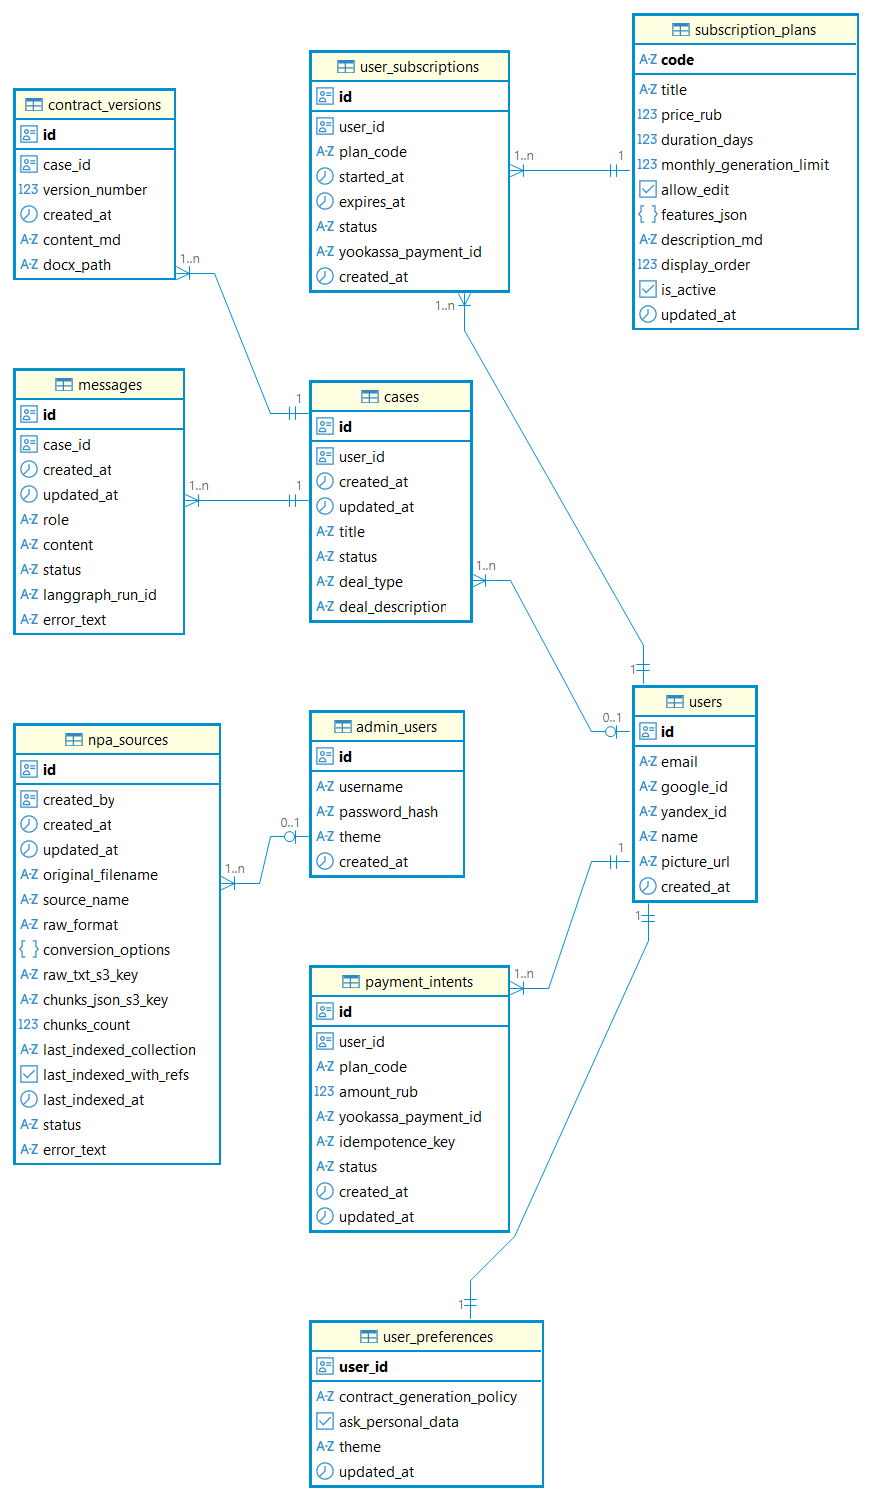
\includegraphics[width=\linewidth,height=0.85\textheight,keepaspectratio]{inc/db_schema}
\caption{ER-диаграмма базы данных программной системы}
\label{fig:er}
\end{figure}

Выбор технологического стека определяется требованиями технического задания (подраздел~1.3) и характером формальной модели агента. LangGraph выбран как фреймворк, наиболее соответствующий предложенной модели: линейные цепочки библиотеки LangChain не поддерживают условные переходы, мульти-агентные фреймворки типа CrewAI и AutoGen предназначены для сценариев свободного взаимодействия нескольких ролей, ручная реализация графа на чистом Python потребовала бы повторной реализации механизма прерывания и возобновления. Векторная база данных Qdrant выбрана за поддержку фильтрации по структурированным метаданным (используется при точечной подгрузке актов по графу ссылок), хранение нескольких независимых коллекций (используется для разнесения корпуса) и наличие официального Python-клиента с асинхронной поддержкой. Веб-уровень построен на FastAPI: типизированные схемы через Pydantic, нативный asyncio, готовый WebSocket-стек и автогенерация OpenAPI-спецификации. Реляционная СУБД~--- PostgreSQL~16: гарантии ACID, нужные биллинговой подсистеме, и поле JSONB для гибких полуструктурированных данных. Объектное хранилище~--- MinIO~\cite{minio_docs}: открытая S3-совместимая реализация с подписанными ссылками.

Принципиальное решение о выборе языковой модели~--- использование открытых моделей с возможностью локального исполнения, а не публичных API крупных коммерческих LLM. Это решение обусловлено характером обрабатываемых данных: пользователь передаёт системе персональные сведения (паспортные данные, ИНН, ОГРН, адреса) и описание планируемой сделки, в ряде случаев финансово существенной. Отправка таких данных в публичный API стороннего поставщика означала бы их доступность этому поставщику в режимах, регулируемых его пользовательским соглашением: для большинства коммерческих LLM-сервисов условия по умолчанию допускают использование пользовательских запросов для обучения и улучшения моделей и иных производных целей. Для правовой задачи, в которой содержание запроса само по себе раскрывает имущественные намерения и личные данные сторон, такой режим обработки несовместим с разумными ожиданиями пользователя относительно конфиденциальности. Использование открытой модели снимает эту проблему: модель и веса доступны для локального запуска внутри периметра эксплуатирующей организации без передачи запросов третьим лицам. В текущем развёртывании используется модель \texttt{gemma4:31b-cloud}~--- модель размера~31~миллиард параметров в режиме облачной маршрутизации Ollama, использованная на этапе экспериментальной проверки; архитектура системы при этом не зависит жёстко от Ollama: благодаря OpenAI-совместимости интерфейса возможно подключение и любого другого совместимого провайдера, включая полностью локальный.

Аутентификация пользователей построена на протоколе OAuth~2.0~\cite{rfc6749} через библиотеку \texttt{authlib} для интеграции с Google и собственную реализацию обмена кода авторизации на токен для Яндекс ID. Аутентификация администраторов реализована отдельным контуром с парами имя пользователя и пароль и хешами bcrypt. Обе аутентификации независимы и происходят разными маршрутами, однако используют общую сессионную cookie: ключи \texttt{user\_id} и \texttt{admin\_id} хранятся в ней параллельно, так что вход в одну роль не вытесняет ранее установленную другую~--- одно физическое лицо может удерживать обе роли в одном браузере, пройдя оба входа. Биллинговая подсистема представляет собой замкнутый домен с собственными бизнес-правилами: тарифные планы хранятся в таблице \texttt{subscription\_plans} и редактируются администратором; зарезервированный код \texttt{free} соответствует бесплатному плану с количественным лимитом на генерации и запретом на редактирование, который реализуется на двух уровнях~--- инжекция признака \texttt{allow\_edit=false} в состояние агента и узел программной преграды внутри графа. Платёжный поток реализован через ЮKassa с уникальным ключом идемпотентности на каждое намерение оплаты; выбор именно этого провайдера определяется его PCI~DSS-совместимостью.

Административный контур позволяет управлять корпусом нормативных правовых актов: загруженный администратором текст нормативного акта сохраняется в бакет \texttt{admin-npa} MinIO, далее запускается деление на чанки, и отдельной задачей администратор инициирует индексацию обработанного акта в одну из коллекций Qdrant. Кроме работы с корпусом административный контур позволяет редактировать каталог поддерживаемых типов сделок, управлять тарифными планами и просматривать список учётных записей. Веб-интерфейс пользователя реализован на ванильном JavaScript без сборочного шага: разметка и стили статически отдаются nginx-контейнером, маршрутизация между видами выполняется переключением CSS-видимости, состояние UI собрано в единый объект и обновляется в реакции на WebSocket-события.

\subsection{Экспериментальная оценка и обоснование выбора конфигурации RAG}

Для эмпирического обоснования выбранной конфигурации поиска (подраздел~2.2) была проведена сравнительная оценка пяти конфигураций на размеченном датасете \texttt{gold\_sources.json} объёмом~54~описания сделок. Каждое описание сопровождается тройкой <<тип договора, перечень источников, перечень спецификаций статей>>, представляющей собой эталонный ответ юриста-эксперта на вопрос <<какие нормы релевантны для подготовки договора по этому описанию>>. Пример одной записи датасета приведён на рисунке~\ref{fig:gold-sample}.

\begin{figure}[H]
\begin{lstlisting}[style=promptstyle, language={}]
{
    "initial_request": "У меня магазин, я продаю товары обычным
        людям для личного пользования, нужен договор для таких продаж",
    "contract_type": "договор розничной купли-продажи",
    "sources": [
        {
            "source_name": "ГК РФ",
            "articles": ["454-491"]
        },
        {
            "source_name": "ФЗ О ЗАЩИТЕ ПРАВ ПОТРЕБИТЕЛЕЙ",
            "articles": ["1", "4", "7", "8-12", "16-17", "18-25", "26.1"]
        }
    ]
}
\end{lstlisting}
\caption{Пример записи эталонного датасета \texttt{gold\_sources.json}}
\label{fig:gold-sample}
\end{figure}

Запуск выполнялся в режиме прерывания графа после узла поиска норм; уточняющие вопросы агента симулировались отдельным LLM-вызовом (роль <<человек, описывающий сделку>>), что снимает зависимость от ручного запуска. Для каждого прогона фиксировались решение классификатора, результаты поиска и измеренная задержка узла поиска.

Метрики определены следующим образом. Для каждого описания зафиксирован эталонный список ссылок на нормы в виде набора пар $G = \{g_1, \dots, g_{|G|}\}$, где $g_j = (s_j, a_j)$: $s_j$~--- имя нормативного акта (например, <<ГК РФ>>), $a_j$~--- спецификация статьи в виде одиночного номера или диапазона номеров (например, $454$--$491$). Извлечённые системой чанки образуют упорядоченную последовательность $R_n = (r_1, r_2, \dots)$ для $n$-го описания сделки. Чанк $r_i$ считается релевантным, если найдётся такая спецификация $g_j$, что имя источника чанка после удаления знаков препинания и приведения к нижнему регистру совпадает с $s_j$, а номер статьи чанка либо совпадает с $a_j$ при одиночном номере, либо принадлежит интервалу при диапазоне. Обозначим через $\mathrm{rel}(R_n, k)$ множество релевантных чанков в первых~$k$ позициях выдачи $R_n$; тогда
\begin{equation}
\mathrm{precision}@k = \frac{1}{N}\sum_{n=1}^{N}\frac{|\mathrm{rel}(R_n, k)|}{k},
\end{equation}
\begin{equation}
\mathrm{hit}@k = \frac{1}{N}\sum_{n=1}^{N}\mathbb{1}\bigl[|\mathrm{rel}(R_n, k)| \ge 1\bigr],
\end{equation}
\begin{equation}
\mathrm{accuracy}_{\mathrm{cls}} = \frac{1}{N}\sum_{n=1}^{N}\mathbb{1}\bigl[\hat{t}_n \equiv t_n\bigr],
\end{equation}
где $\hat{t}_n$~--- предсказанный тип сделки, $t_n$~--- эталонный тип, $N$~--- число описаний сделок в выборке. Дополнительно фиксируется $\mathrm{latency}$~--- задержка узла поиска норм, измеренная в миллисекундах как суммарное время от подачи запроса в узел до возврата итоговой выдачи; в сводных результатах приводятся среднее ($\mathrm{latency}_{\mathrm{mean}}$), медиана ($\mathrm{latency}_{\mathrm{median}}$) и 90-й перцентиль ($\mathrm{latency}_{\mathrm{p90}}$) распределения значений по выборке.

Каждая из введённых величин отражает свой аспект качества поиска. Метрика $\mathrm{precision}@k$ показывает, какая доля норм в первых~$k$ позициях выдачи действительно релевантна запросу: чем выше значение, тем меньше постороннего материала попадает в контекст языковой модели и тем меньше риск, что он исказит ответ. Метрика $\mathrm{hit}@k$ показывает, в какой доле запросов среди первых~$k$ позиций нашлась хотя бы одна релевантная норма; значение, равное единице, означает, что ни один запрос не остался без нужного контекста. Метрика $\mathrm{accuracy}_{\mathrm{cls}}$ показывает долю верно определённых типов сделок и отражает надёжность ветвления в графе агента до запуска поиска: ошибка классификации направит запрос не в ту коллекцию норм. Величина $\mathrm{latency}$ задаёт практический компромисс конфигурации поиска: каждая дополнительная ступень~--- реранкер, LLM-фильтр~--- повышает $\mathrm{precision}@k$ и $\mathrm{hit}@k$, но удлиняет обработку, и в отбор оптимальной связки приходится включать ограничение по приемлемому для пользователя времени отклика. Высокое значение $\mathrm{precision}@k$ вместе с высоким $\mathrm{accuracy}_{\mathrm{cls}}$, единичным $\mathrm{hit}@k$ и удержанием $\mathrm{latency}$ в пределах целевого ограничения по времени отклика означает, что в выдаче поиска одновременно присутствует нужный ответ, отсутствует посторонний шум, способный исказить генерацию, а сам поиск укладывается во временной бюджет сценария.

Сравнивались пять конфигураций, представляющих разумные варианты двухступенчатого поиска (во всех использовалась модель эмбеддингов \texttt{ai-sage/Giga-Embeddings-instruct} в режиме \texttt{bfloat16}, различия касаются второго этапа~--- реранкера и LLM-фильтра): базовая (только бикодер); бикодер~$+$ реранкер \texttt{BAAI/bge-reranker-v2-m3}; бикодер~$+$ \texttt{bge-reranker-v2-m3}~$+$ LLM-фильтр; бикодер~$+$ \texttt{Qwen/Qwen3-Reranker-0.6B}; бикодер~$+$ \texttt{Qwen3-Reranker-0.6B}~$+$ LLM-фильтр (текущая). Результаты сведены в таблице~\ref{tab:eval-comparison}.
\begin{table}[H]
\caption{Сравнение пяти конфигураций поиска (метрики качества~--- в процентах; latency~--- в миллисекундах; жирным выделено лучшее значение в каждой строке: максимум для метрик качества, минимум для latency)}
\label{tab:eval-comparison}
\renewcommand{\arraystretch}{1.20}
\setlength{\tabcolsep}{4pt}
\footnotesize
\begin{tabularx}{\textwidth}{|>{\raggedright\arraybackslash}X|c|c|c|c|c|} \hline
\textbf{Метрика} & \textbf{\#1} & \textbf{\#2} & \textbf{\#3} & \textbf{\#4} & \textbf{\#5} \\ \hline
$\mathrm{accuracy}_{\mathrm{cls}}$ & 100 & 100 & 100 & 100 & 100 \\ \hline
$\mathrm{precision}@3$ & 42.6 & 77.8 & 85.8 & 85.8 & \textbf{91.4} \\ \hline
$\mathrm{hit}@3$ & 81.5 & 98.1 & 98.1 & 98.1 & \textbf{100.0} \\ \hline
$\mathrm{precision}@5$ & 41.1 & 71.5 & 82.2 & 81.5 & \textbf{89.6} \\ \hline
$\mathrm{hit}@5$ & 90.7 & 98.1 & 98.1 & 98.1 & \textbf{100.0} \\ \hline
$\mathrm{precision}@10$ & 38.0 & 64.4 & 69.3 & 70.2 & \textbf{78.0} \\ \hline
$\mathrm{hit}@10$ & \textbf{100.0} & 98.1 & 98.1 & 98.1 & \textbf{100.0} \\ \hline
$\mathrm{precision}@20$ & 27.6 & 46.7 & 42.3 & \textbf{48.8} & 47.8 \\ \hline
$\mathrm{hit}@20$ & \textbf{100.0} & 98.1 & 98.1 & 98.1 & \textbf{100.0} \\ \hline
$\mathrm{latency}_{\mathrm{mean}}$ & \textbf{243} & 2050 & 9766 & 4309 & 13644 \\ \hline
$\mathrm{latency}_{\mathrm{median}}$ & \textbf{204} & 1788 & 7124 & 4072 & 8542 \\ \hline
$\mathrm{latency}_{\mathrm{p90}}$ & \textbf{461} & 3901 & 17073 & 5714 & 29173 \\ \hline
\end{tabularx}
\end{table}

Полученные значения метрик демонстрируют поступательное улучшение качества поиска с каждым дополнительным компонентом конвейера. Базовая конфигурация~\#1 (только бикодер) обеспечивает попадание релевантной нормы в первые три позиции выдачи в~81.5~\% случаев. Подключение кросс-энкодерного реранкера (конфигурация~\#2) повышает $\mathrm{precision}@3$ с~42.6~\% до~77.8~\% (рост в~1.83~раза), а $\mathrm{hit}@3$~--- с~81.5~\% до~98.1~\%, что согласуется с известным свойством двухступенчатого поиска: бикодер обеспечивает охват, кросс-энкодер дотягивает точность ранжирования верхушки выдачи. Дальнейшее подключение LLM-фильтра поверх классического реранкера BGE (конфигурация~\#3) даёт дополнительный точностный прирост ($\mathrm{precision}@3 = 85.8$~\%); замена реранкера на современный Qwen3-Reranker-0.6B без фильтра (конфигурация~\#4) обеспечивает аналогичный точностный уровень при меньшей задержке отклика. Итоговая конфигурация~\#5, объединяющая Qwen3-Reranker-0.6B с LLM-фильтром, достигает наилучших показателей по всем целевым метрикам верхушки выдачи: $\mathrm{hit}@3 = 100$~\%, $\mathrm{precision}@3 = 91.4$~\%, $\mathrm{precision}@5 = 89.6$~\%, $\mathrm{precision}@10 = 78.0$~\%. На границе $k = 20$ точностный выигрыш LLM-фильтра нивелируется: значение $\mathrm{precision}@20 = 47.8$~\% в~\#5 несущественно ниже $48.8$~\% в~\#4 без фильтра, что объясняется естественной ограниченностью пользы фильтрации на длинном хвосте выдачи. Latency узла поиска ожидаемо растёт с каждой дополнительной ступенью обработки: от $\mathrm{latency}_{\mathrm{mean}} = 243$~мс в базовой конфигурации до $13.6$~с в итоговой; медианное значение составляет $8.5$~с, тогда как $\mathrm{latency}_{\mathrm{p90}}$ доходит до $29.2$~с~--- это указывает на длинный правый хвост распределения, обусловленный кейсами, на которых LLM-фильтр обрабатывает увеличенное число батчей. Метрики итоговой конфигурации в детализированном виде по всем рассматриваемым значениям~$k$ приведены на рисунке~\ref{fig:eval-best}.

\begin{figure}[H]
\centering
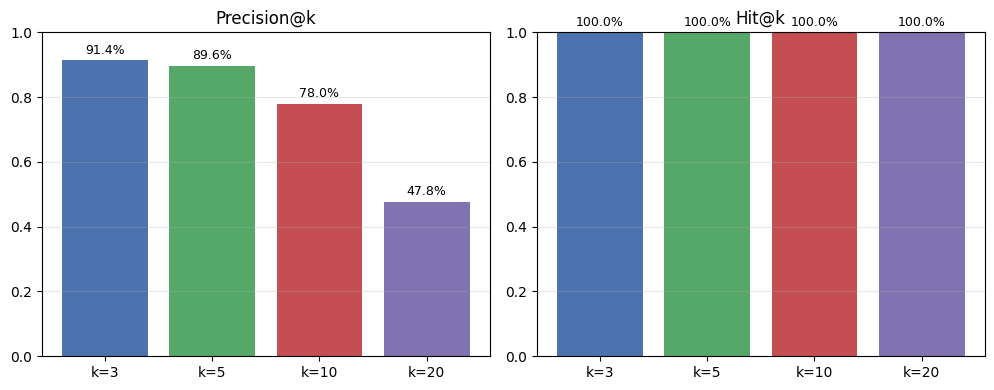
\includegraphics[width=0.95\linewidth]{inc/eval_best_metrics}
\caption{Метрики итоговой конфигурации~\#5: $\mathrm{precision}@k$ и $\mathrm{hit}@k$ для $k \in \{3, 5, 10, 20\}$}
\label{fig:eval-best}
\end{figure}

Приведённые на рисунке~\ref{fig:eval-best} значения~--- усреднённые по всему набору из~54~описаний сделок. Распределение тех же метрик в разрезе типов договоров приведено на рисунке~\ref{fig:eval-heatmap}: $\mathrm{accuracy}_{\mathrm{cls}}$ достигает значения 100~\% для каждого из представленных типов сделок, оценки $\mathrm{precision}@3$ сосредоточены в верхней зоне шкалы, а при росте~$k$ распределение значений ожидаемо смещается вниз~--- естественное следствие более строгого требования к попаданию релевантной нормы в большее число позиций выдачи.

\begin{figure}[H]
\centering
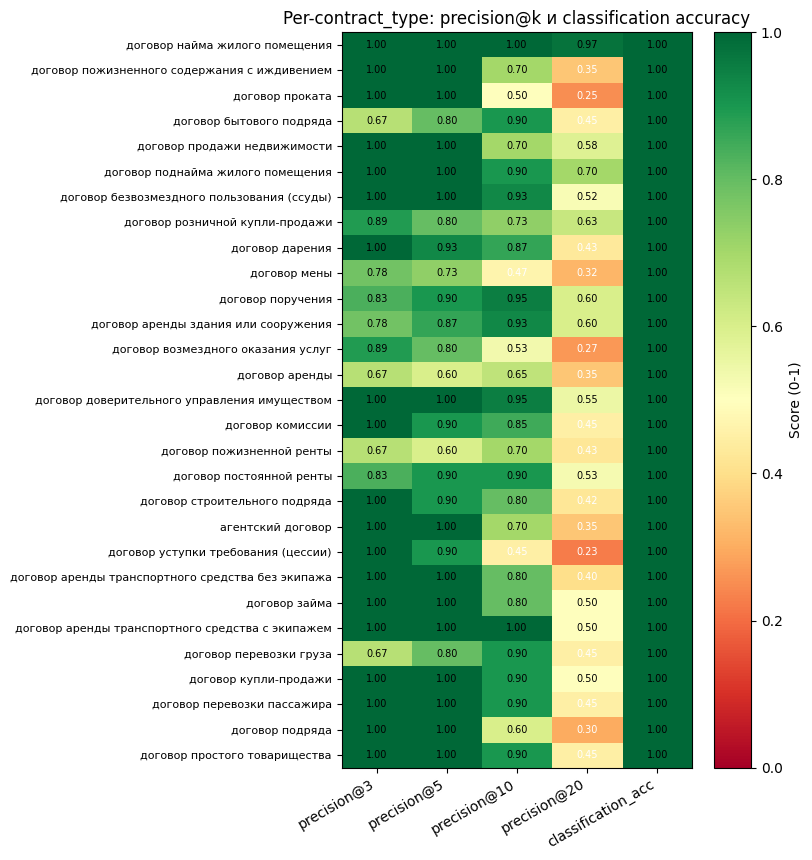
\includegraphics[width=0.85\linewidth]{inc/eval_heatmap}
\caption{Распределение значений $\mathrm{precision}@k$ и $\mathrm{accuracy}_{\mathrm{cls}}$ итоговой конфигурации поиска по типам сделок}
\label{fig:eval-heatmap}
\end{figure}

Точность классификации сделки во всех конфигурациях составляет 100~\%, что объясняется надёжностью двухступенчатой стратегии классификатора (основной классификатор плюс субагент с RAG-поддержкой при низкой уверенности в ответе) на коротких словесных описаниях. Достигнутый уровень метрик соответствует целевой постановке задачи: стопроцентный $\mathrm{hit}@3$ означает, что нижестоящие узлы графа гарантированно получают релевантную норму в составе своего контекста, а $\mathrm{precision}@3 = 91.4$~\% обеспечивает, что верхушка выдачи практически полностью состоит из применимых норм и не загрязняет вход LLM шумом. Замеренная задержка узла поиска в~13.6~с приемлема для целевого сценария подготовки договора, где пользователь ожидает результат на временной шкале десятков секунд. По совокупности результатов в качестве рабочей конфигурации поиска принята связка \texttt{ai-sage/Giga-Embeddings-instruct}~+ \texttt{Qwen/Qwen3-Reranker-0.6B}~+ LLM-фильтр на батчах размера~10.

\section{РЕЗУЛЬТАТЫ РАЗРАБОТКИ}

В настоящей главе представлены результаты разработки: целевые условия и сценарии применения системы, демонстрация её работы на типовом пользовательском сценарии, итоги внешней экспертной оценки качества подготавливаемых артефактов и сводные технические характеристики решения.

\subsection{Условия и сценарии практического применения разработанной системы}

Разработанная система ориентирована на физических лиц и субъектов малого предпринимательства, заключающих типовые сделки гражданского оборота (подробное обоснование~--- в подразделе~1.1). Целевая предметная область~--- поименованные в ГК~РФ сделки гражданского оборота, типичные для бытовой практики и для оборота малого бизнеса. Конкретный перечень поддерживаемых типов договоров не зафиксирован в исходном коде, а определяется составом проиндексированного корпуса нормативных правовых актов: администратор через панель управления загружает источники в индекс и регистрирует соответствующие типы сделок в каталоге без перекомпиляции приложения (механизм рассмотрен в подразделе~2.3). Тем самым система адаптивна по охвату: эксплуатирующая организация настраивает поддерживаемые типы сделок под собственный сценарий применения. Корпоративные сделки со сложным предметом, сделки с особым нотариальным режимом и сделки с публичными элементами выходят за пределы целевой постановки задачи.

Режим доступа~--- web-интерфейс с входом через внешних провайдеров идентификации (Google или Яндекс по протоколу OAuth~2.0). Тарификация двухуровневая: бесплатный план с количественным лимитом и без возможности редактирования сгенерированного документа; платные планы снимают эти ограничения. Оплата осуществляется через ЮKassa. Принципиальный режим эксплуатации~--- сохранение конфиденциальности данных пользователя: при локальном развёртывании архитектура не предполагает передачи сведений третьим лицам (см. подраздел~2.3).

\subsection{Демонстрация работы агента в типовом сценарии}

Типовой пользовательский сценарий охватывает последовательность шагов от описания сделки до получения готового пакета документов. После аутентификации пользователь формулирует словесное описание планируемой сделки в свободной форме (например: <<хочу сдать однокомнатную квартиру в Москве на 11~месяцев, арендатор~--- физическое лицо>>); сообщение поступает в эндпоинт \texttt{POST /api/chat} и обрабатывается графом состояний агента (подраздел~2.1). Если описание недостаточно для согласования существенных условий, узел проверки достаточности данных формирует уточняющий вопрос и приостанавливает граф через сохранение контрольного пункта; следующее сообщение пользователя возобновляет обработку с того же узла. Пример диалогового взаимодействия приведён на рисунке~\ref{fig:demo-chat-dialog}.

\begin{figure}[H]
\centering
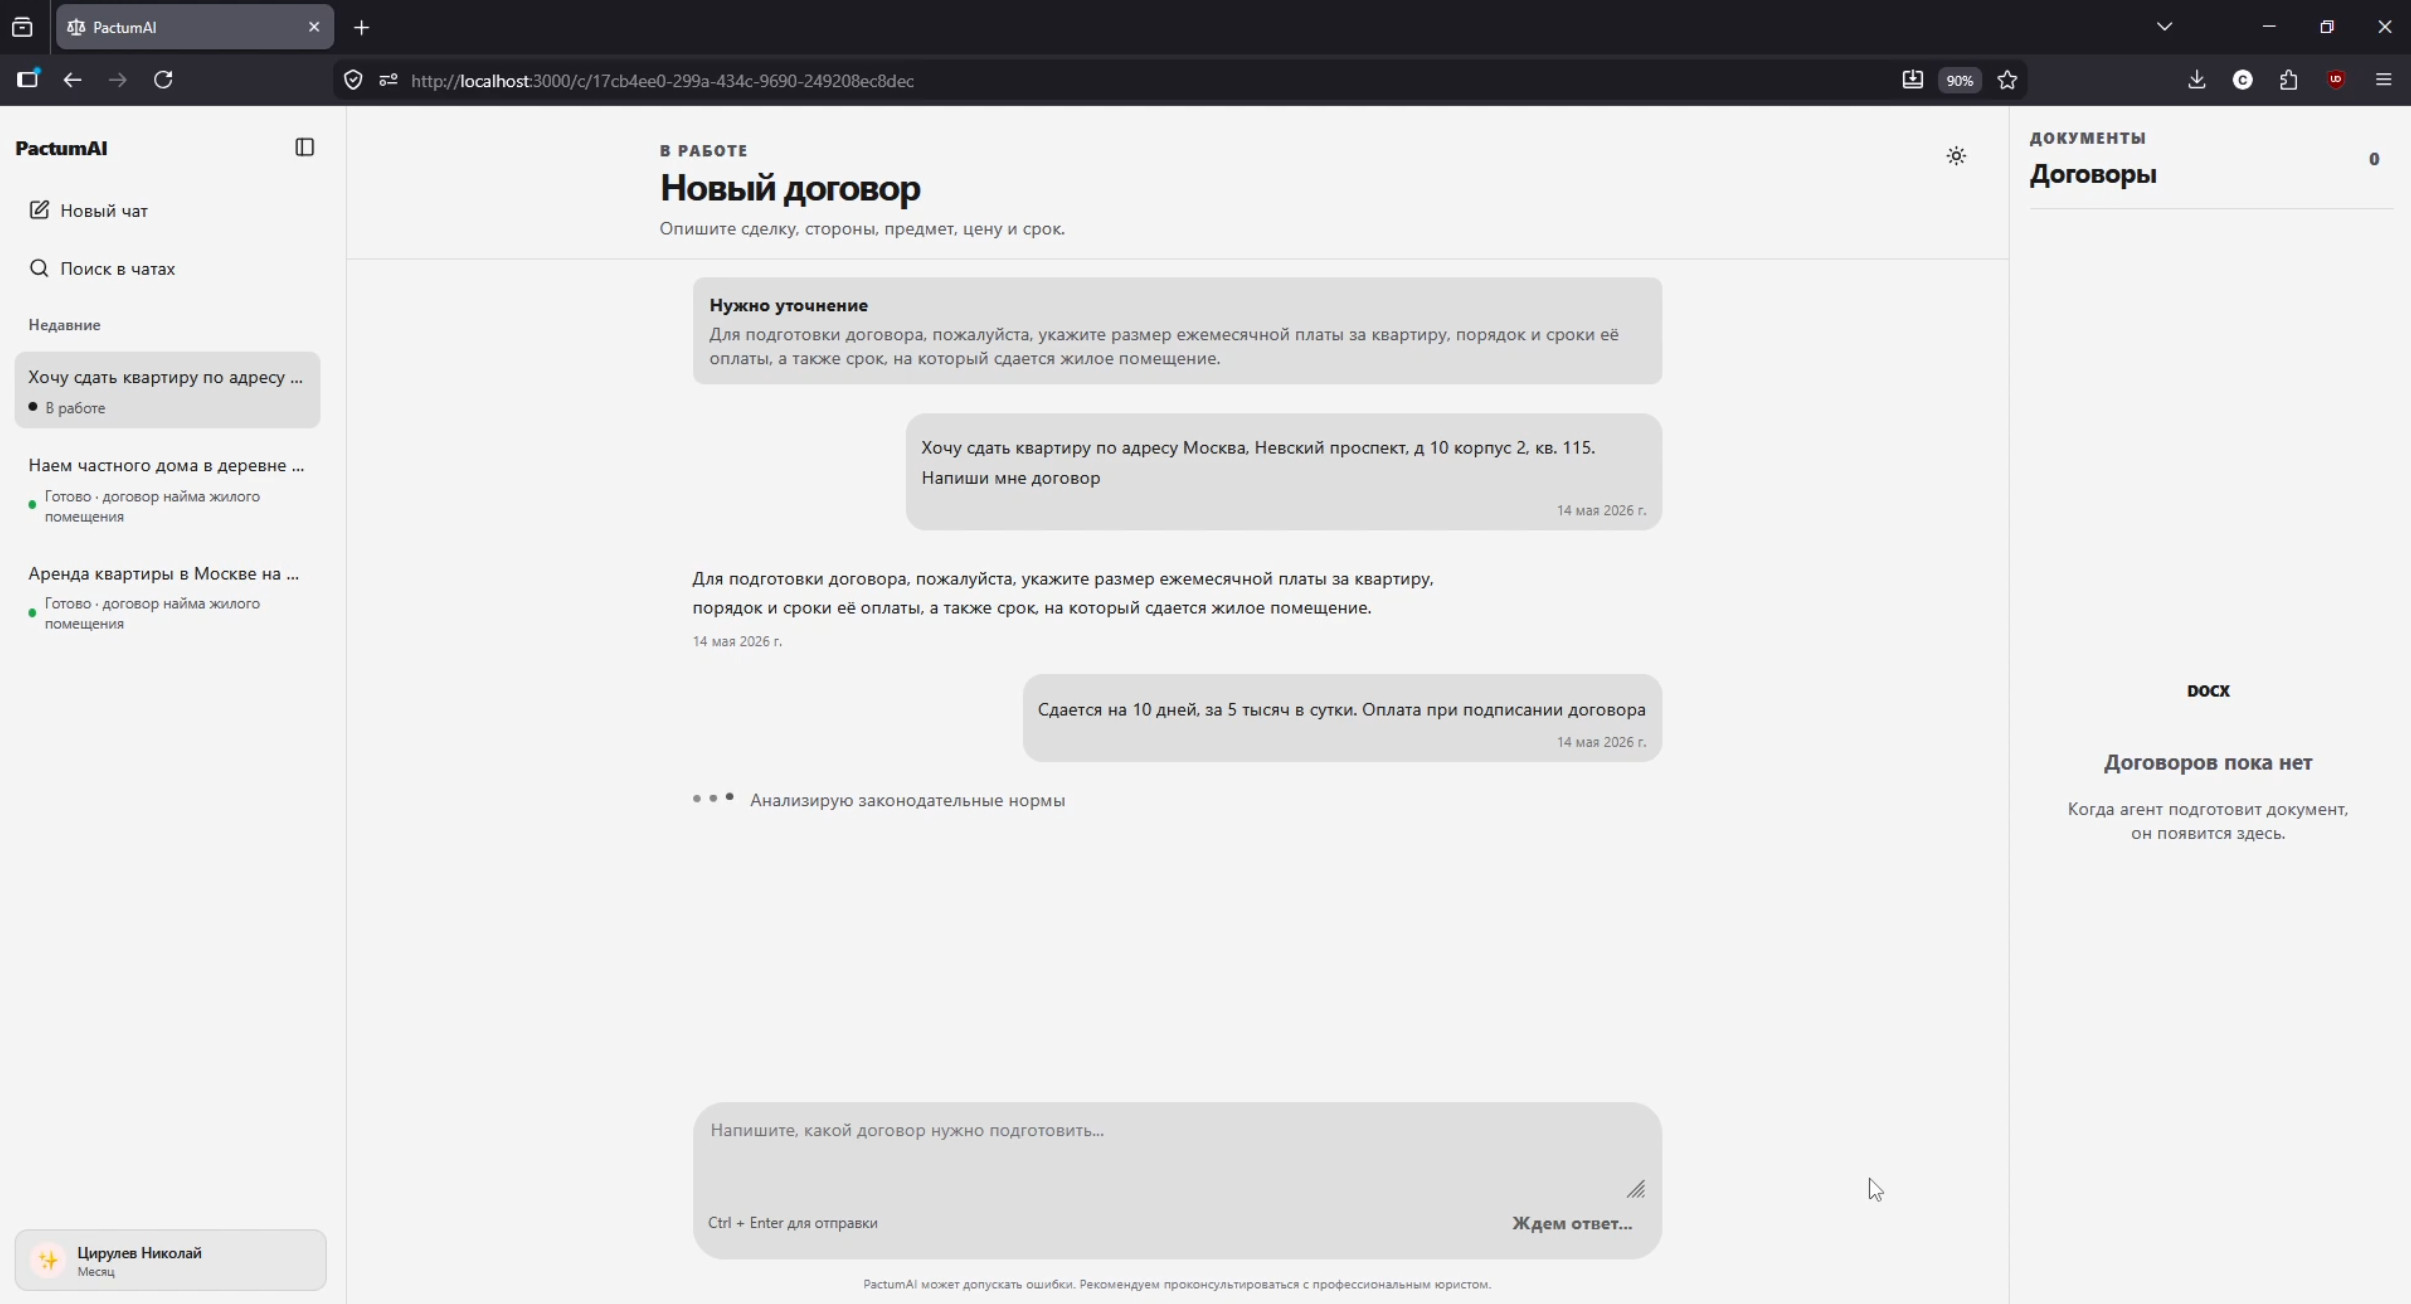
\includegraphics[width=0.9\linewidth]{inc/chat_dialog}
\caption{Окно чата с типовым диалогом: запрос пользователя, уточняющий вопрос агента и ответ пользователя}
\label{fig:demo-chat-dialog}
\end{figure}

После сбора существенных сведений граф последовательно выполняет проверку правовой допустимости сделки по общим нормам, поиск релевантных норм по корпусу нормативных правовых актов, генерацию проекта договора и его автоматическую итеративную валидацию (подразделы~2.1 и~2.2). Узел формирования рекомендаций выдаёт юридический отчёт со ссылками на статьи нормативных правовых актов в формате \texttt{[Источник, статья]}, а узел сохранения результата конвертирует проект договора в DOCX-файл и публикует ссылку для скачивания; внешний вид окна чата на этом этапе приведён в приложении~Д (рисунок~\ref{fig:app-chat-recs}).

Сгенерированный проект оформлен в типовой структуре делового документа: реквизиты сторон, девять содержательных разделов (предмет; срок действия; права и обязанности сторон; цена и порядок расчётов; ответственность; изменение и расторжение; разрешение споров; заключительные положения; реквизиты и подписи) и поля для рукописного заполнения недостающих сведений; шрифт Times~New~Roman 12~пт, полуторный межстрочный интервал, поля по 25~мм. Пример страницы приведён на рисунке~\ref{fig:demo-contract-page}.

\begin{figure}[H]
\centering
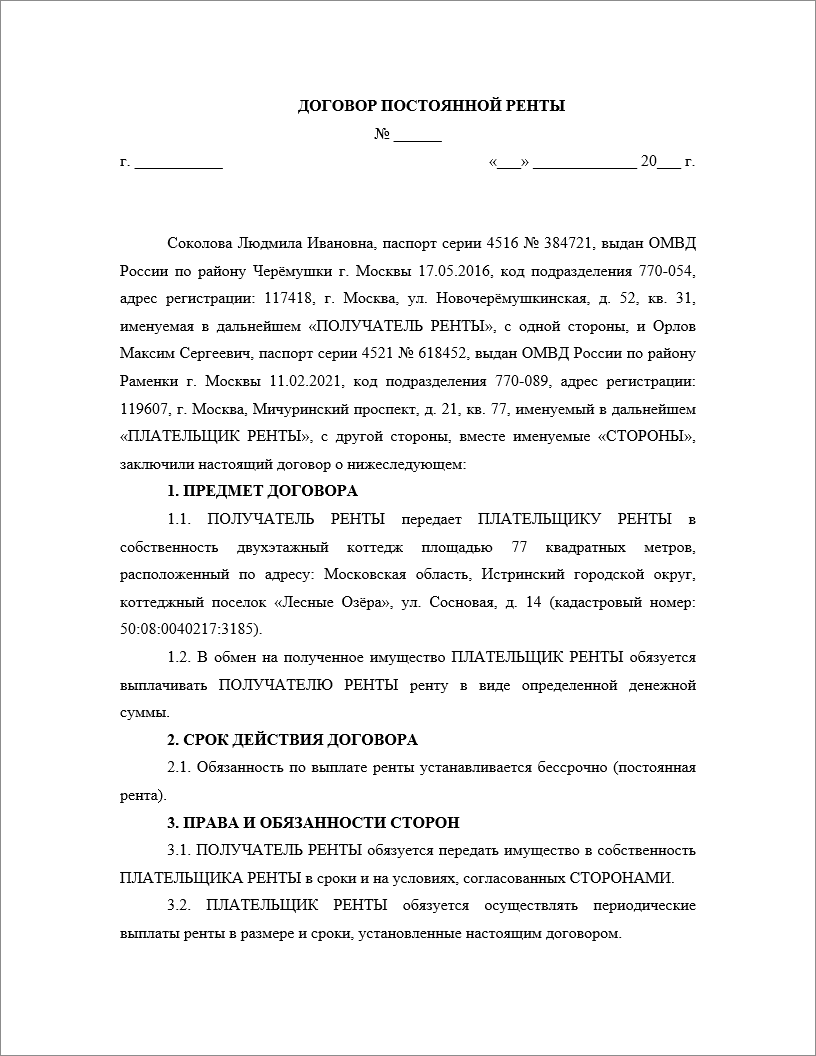
\includegraphics[width=0.85\linewidth]{inc/contract_docx_page}
\caption{Содержательная страница сгенерированного проекта договора в формате DOCX}
\label{fig:demo-contract-page}
\end{figure}

Помимо основного сценария генерации пользователь имеет доступ к двум вспомогательным экранам, не связанным напрямую с процессом подготовки договора и потому вынесенным в приложение~Д. Окно настроек (рисунок~\ref{fig:app-user-prefs}) позволяет управлять режимом генерации проекта договора (варианты <<всегда>>, <<только при предусмотренной законом письменной форме>>, <<уточнять у пользователя>>) и обращением с персональными данными (запрашивать конкретные значения у пользователя либо подставлять в проект договора плейсхолдеры для последующего ручного заполнения). Страница тарифов (рисунок~\ref{fig:app-user-billing}) показывает текущий план пользователя и доступные подписки; переход к оплате ведёт в платёжный шлюз ЮKassa (см. подраздел~2.3).

Параллельно с пользовательским контуром в системе развёрнут административный контур, реализующий жизненный цикл нормативного корпуса и управление каталогом продукта. На вкладке загрузки администратор перетаскивает один или несколько TXT-файлов нормативных правовых актов и при необходимости включает обнаружение перекрёстных ссылок между статьями~--- последнее замедляет загрузку, но позволяет агенту в дальнейшем расширять результат поиска по графу взаимных ссылок (см. подраздел~2.2). Внешний вид вкладки приведён на рисунке~\ref{fig:demo-admin-upload}. После завершения серверной обработки источник появляется в списке загруженных НПА (рисунок~\ref{fig:demo-admin-sources}); для каждой записи отображаются имя файла-источника, число выделенных чанков, дата загрузки, статус обработки (<<готов к индексации>>, <<индексация>>, <<проиндексирован>>) и кнопки выгрузки исходного текста и JSON-представления чанков. Администратор отмечает один или несколько источников галочками и индексирует их в выбранную коллекцию Qdrant~--- общие, специальные или дополнительные нормы; флажок очистки индекса позволяет переиндексировать источник заново в случае внесённых правок в чанкование.

\begin{figure}[H]
\centering
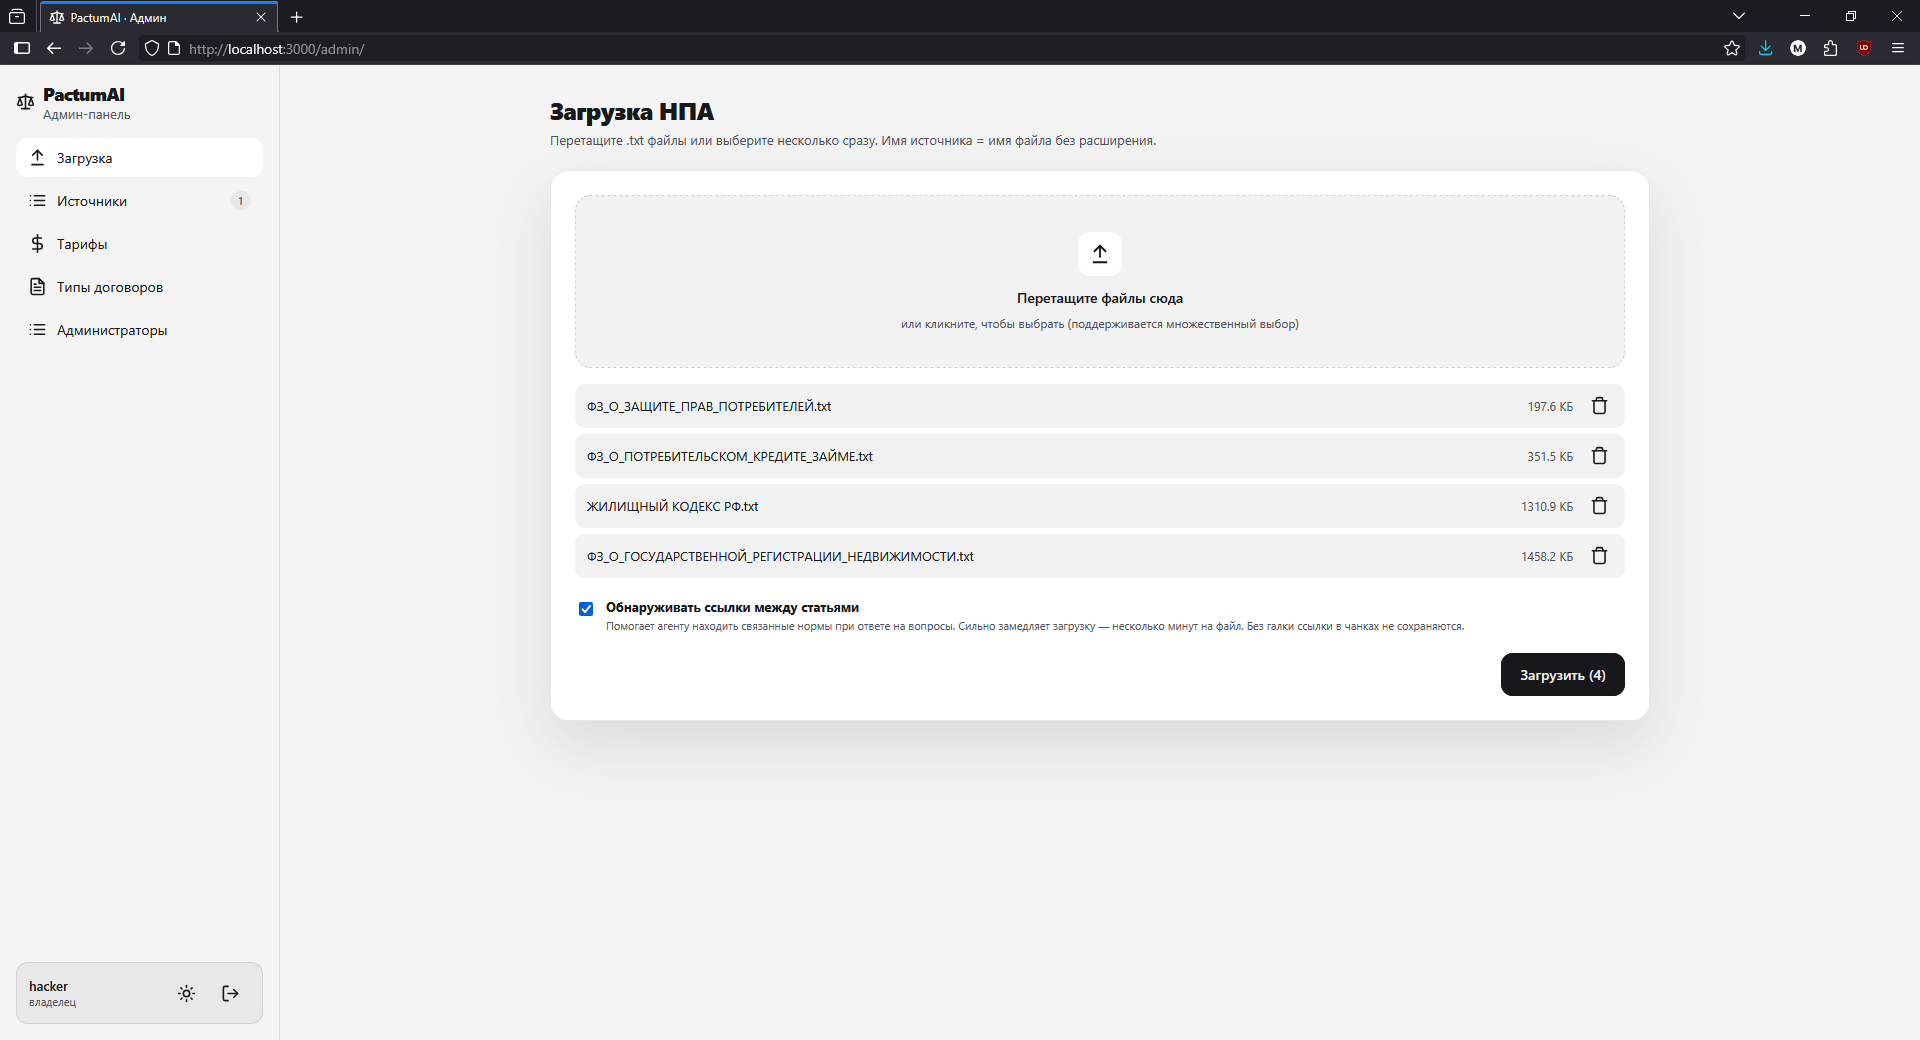
\includegraphics[width=0.9\linewidth]{inc/admin_upload}
\caption{Вкладка <<Загрузка>> административной панели: пакетное добавление нормативных правовых актов с опцией обнаружения перекрёстных ссылок между статьями}
\label{fig:demo-admin-upload}
\end{figure}

\begin{figure}[H]
\centering
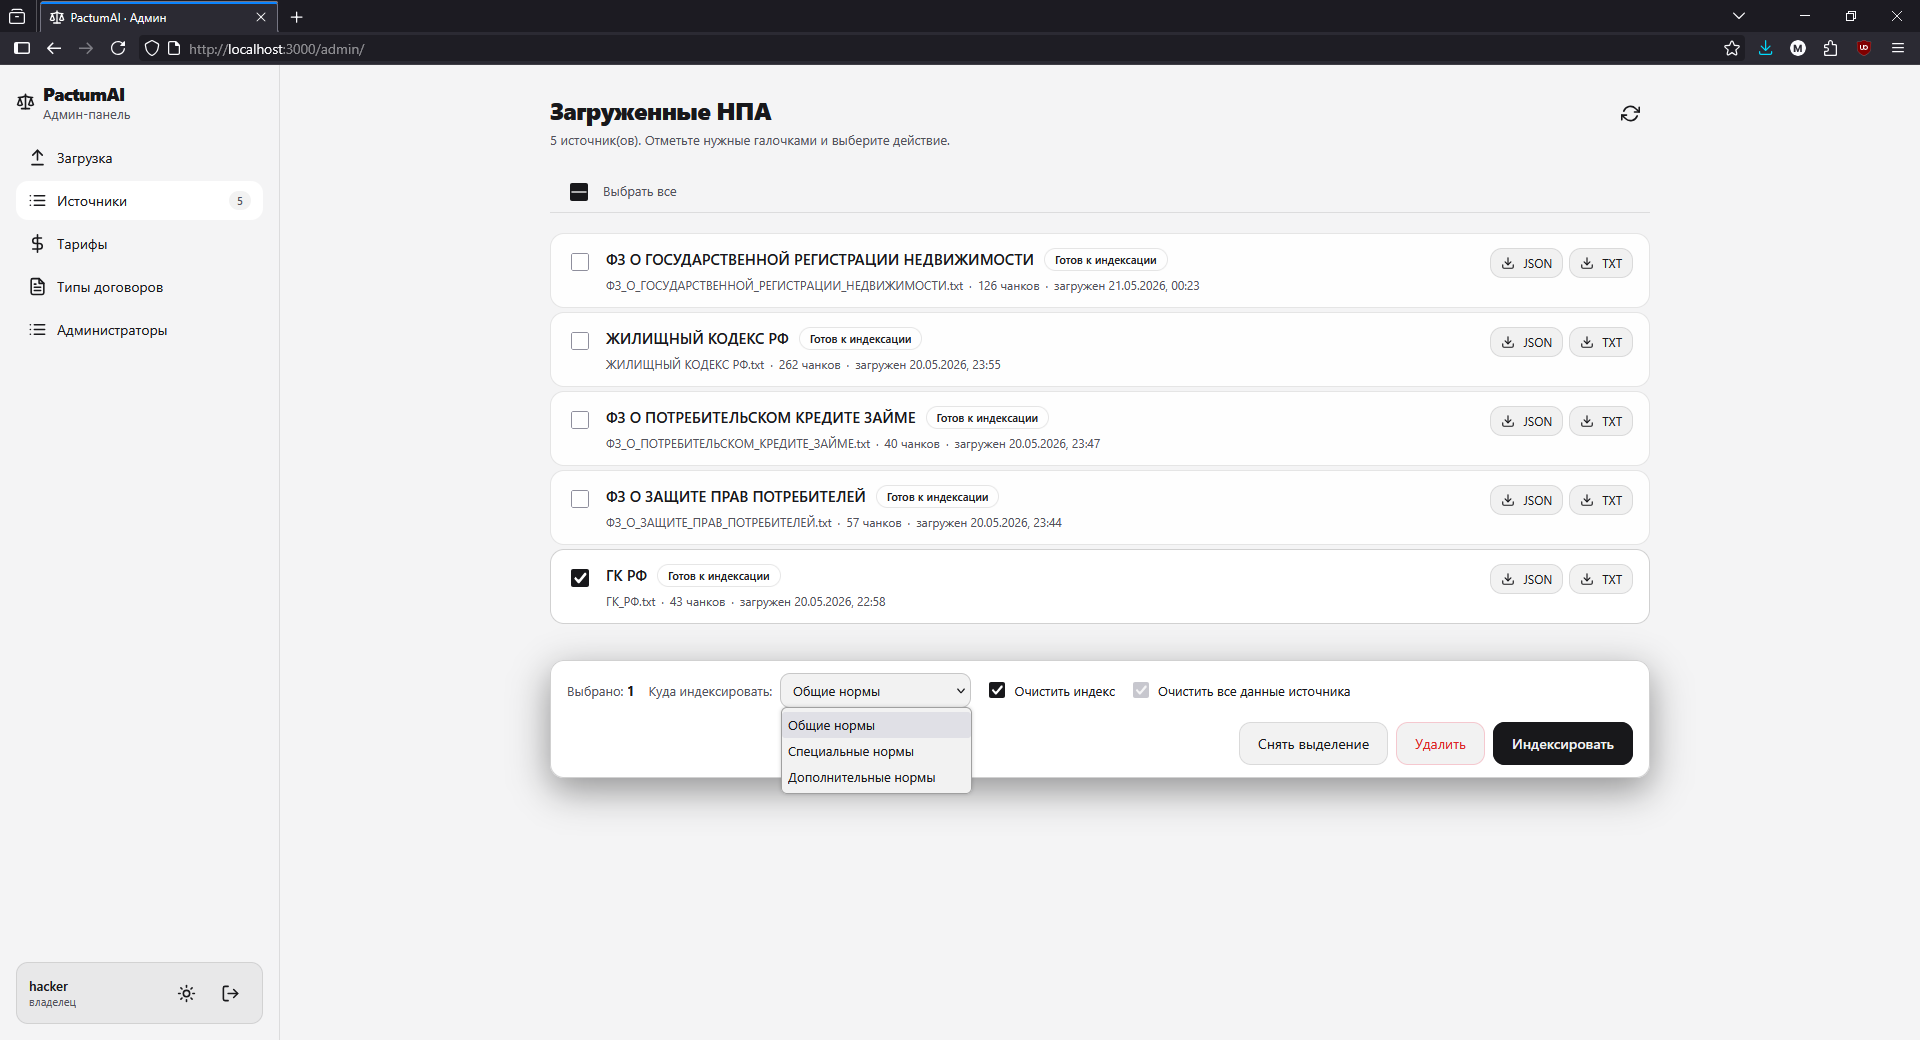
\includegraphics[width=0.9\linewidth]{inc/admin_sources}
\caption{Вкладка <<Источники>>: список загруженных нормативных правовых актов со статусами обработки и панель действий для индексации в выбранную коллекцию}
\label{fig:demo-admin-sources}
\end{figure}

Помимо работы с корпусом, административная панель включает редактор каталога поддерживаемых типов сделок и редактор тарифных планов; внешний вид этих экранов приведён в приложении~Д (рисунки~\ref{fig:app-admin-deal-types}, \ref{fig:app-admin-tariffs} и~\ref{fig:app-admin-tariffs-preview}). Каталог типов сделок хранится в JSON-формате в объектном хранилище и применяется графом агента в течение нескольких секунд после сохранения~--- без перекомпиляции и без перезапуска контейнеров. Редактор тарифов позволяет создавать и изменять планы (цена в рублях, длительность подписки в днях, месячный лимит генераций, разрешение на правку договора в чате, видимость плана для пользователей), включая редактирование Markdown-описания, отображаемого на пользовательской странице тарифов; кнопка предпросмотра открывает модальное окно с пользовательским видом страницы тарифов в текущем состоянии редактора, что позволяет администратору сверить итоговый вид перед сохранением.

\subsection{Экспертная оценка качества подготовленных артефактов}

Для качественной оценки разработанной системы проведена внешняя экспертная апробация с привлечением трёх практикующих юристов. Все привлечённые эксперты в анкетных сведениях указали высшее юридическое образование, полученное в Московском государственном юридическом университете имени О.Е.~Кутафина (МГЮА) по специальности <<Юриспруденция>>. Постановка исследования: эксперту-юристу предъявляются готовые артефакты системы~--- сгенерированный проект договора и сопровождающие юридические рекомендации,~--- и эксперт независимо оценивает их по принятой шкале. Размер выборки соответствует характеру исследования: проведённая оценка имеет характер апробации, а не статистически достоверного экспертного исследования. Инструмент сбора оценок~--- web-форма опроса, размещённая на платформе \texttt{form.jotform.com}. На первой странице формы помещена преамбула об обезличенности полученных результатов и собираются анкетные сведения об эксперте (полученное образование, специальность и стаж практической работы в юридической сфере). На каждой из последующих страниц рассматривается один кейс: эксперту предъявляется пользовательское описание сделки, выданные системой юридические рекомендации и проект договора в формате DOCX, после чего по каждому артефакту выставляется оценка по принятой шкале.

Шкала оценки~--- пятибалльная шкала Лайкерта~\cite{likert1932} с подписанными якорями: 1~--- критически неприемлемо; 2~--- слабо; 3~--- удовлетворительно; 4~--- хорошо; 5~--- отлично, можно использовать. Сбор оценок проводился по двум показателям~--- качество сгенерированного проекта договора и качество сопровождающих юридических рекомендаций. Массив кейсов составили одиннадцать модельных сделок, охватывающих представительный для бытовой практики набор поименованных в ГК~РФ типов договоров (купля-продажа, продажа недвижимости, дарение, мена, заём, аренда, прокат, наём жилого помещения, подряд, возмездное оказание услуг, агентский договор); три эксперта независимо оценивали каждый кейс по двум показателям, что даёт массив из 66~оценок.

Полученные оценки полностью попадают в верхнюю половину шкалы~--- ни один артефакт не был оценён ниже уровня <<хорошо>>. Распределение оценок приведено в таблице~\ref{tab:expert-distribution}, средние~--- в таблице~\ref{tab:expert-means}.

\begin{table}[H]
\caption{Распределение полученных оценок по показателям}
\label{tab:expert-distribution}
\renewcommand{\arraystretch}{1.20}
\begin{tabularx}{\textwidth}{|>{\raggedright\arraybackslash}X|c|c|c|c|} \hline
\textbf{Показатель} & \textbf{<<4>>, шт.} & \textbf{<<5>>, шт.} & \textbf{<<4>>, \%} & \textbf{<<5>>, \%} \\ \hline
Качество проекта договора & 19 & 14 & 57.6 & 42.4 \\ \hline
Качество рекомендаций & 9 & 24 & 27.3 & 72.7 \\ \hline
\end{tabularx}
\end{table}

\begin{table}[H]
\caption{Средние оценки по экспертам и показателям}
\label{tab:expert-means}
\renewcommand{\arraystretch}{1.20}
\begin{tabularx}{\textwidth}{|>{\raggedright\arraybackslash}X|c|c|c|} \hline
\textbf{Эксперт} & \textbf{Качество договора} & \textbf{Качество рекомендаций} & \textbf{Разница} \\ \hline
Эксперт~1 & 4.36 & 4.55 & 0.19 \\ \hline
Эксперт~2 & 4.45 & 4.73 & 0.28 \\ \hline
Эксперт~3 & 4.45 & 4.91 & 0.46 \\ \hline
\textbf{В среднем} & \textbf{4.42} & \textbf{4.73} & \textbf{0.31} \\ \hline
\end{tabularx}
\end{table}

Средняя оценка качества проекта договора по выборке составила 4.42, средняя оценка качества рекомендаций~--- 4.73. Систематическая разница в пользу рекомендаций воспроизводится у каждого из трёх экспертов и объясняется содержательной разницей задач, решаемых двумя артефактами. Качество рекомендаций определяется прежде всего корректностью идентификации применимых норм и сопровождающих сделку рисков; LLM в режиме генерации, дополненной поиском по проиндексированному корпусу, надёжно подсвечивает существенные условия и сопровождает каждое утверждение проверяемой ссылкой на статью нормативного акта, что и фиксируется экспертами в верхней части шкалы. Подготовка проекта договора предъявляет к системе дополнительное требование~--- воспроизведение традиционной для данного типа сделки структуры и формулировок, которая не закреплена в законе, а сложилась в правоприменительной практике. Большинство свободных комментариев экспертов по проекту договора фиксировало именно этот аспект: документ оценивался как юридически корректный, но менее привычный по форме, чем типовой образец, который применил бы практикующий юрист. Расширение библиотеки типовых шаблонов договоров позволит при сохранении единого ядра системы порождать документ ожидаемой для каждого типа сделки структуры без отступления от его юридической корректности; настоящая работа использует единый универсальный шаблон, и развитие библиотеки типовых шаблонов выделено в направление дальнейшей работы. Распределение оценок по типам сделок приведено на рисунках~\ref{fig:expert-contract} и~\ref{fig:expert-recs}: оценки удерживаются в диапазоне $[4.0,\,5.0]$ для всех одиннадцати рассмотренных типов договоров.

\begin{figure}[H]
\centering
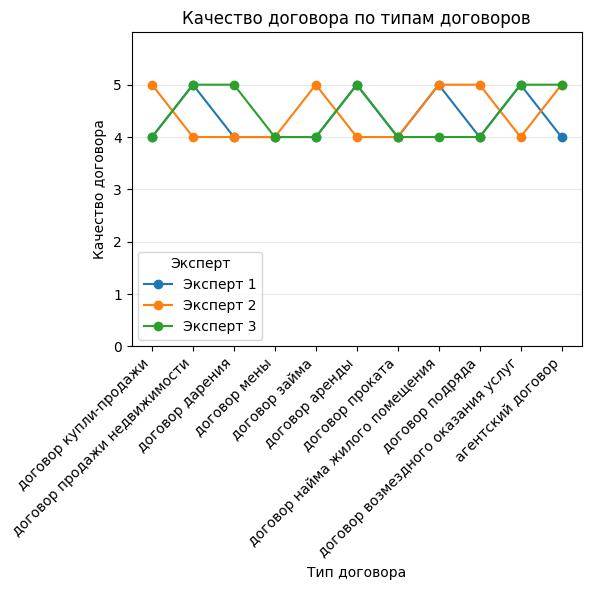
\includegraphics[width=0.85\linewidth]{inc/expert_quality_contract}
\caption{Оценки качества проекта договора по типам договоров (одна линия~--- один эксперт)}
\label{fig:expert-contract}
\end{figure}

\begin{figure}[H]
\centering
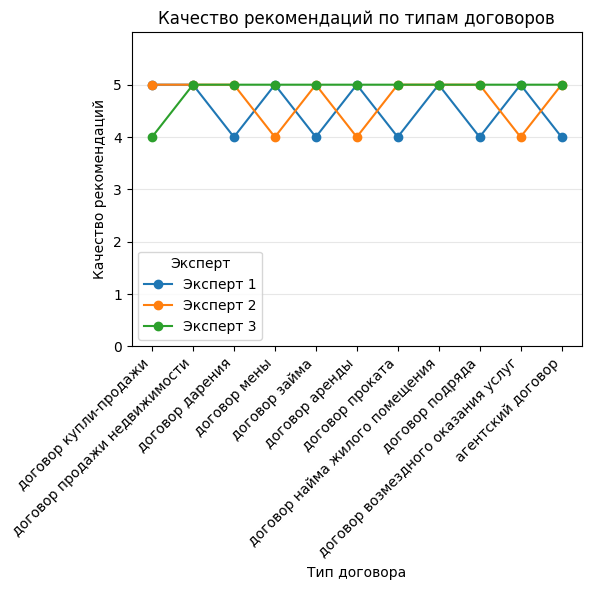
\includegraphics[width=0.85\linewidth]{inc/expert_quality_recs}
\caption{Оценки качества рекомендаций по типам договоров (одна линия~--- один эксперт)}
\label{fig:expert-recs}
\end{figure}

Ограничения проведённого исследования: выборка из трёх экспертов носит характер апробации; интегральная двухосевая оценка не разделяет ответственность за итоговый результат между подсистемами агента. Направления дальнейшего развития исследования~--- увеличение экспертной выборки и развёртывание оценки на несколько раздельных показателей (корректность ссылок на нормы права, полнота существенных условий, структурная корректность договора).

\subsection{Технические характеристики разработанного решения}

Сводные технические характеристики приведены в таблице~\ref{tab:tech-summary}. Производительность системы удерживается в рамках поставленного в подразделе~1.3 требования о среднем времени отклика в пределах единиц минут на полный цикл подготовки документа; доминирующий вклад в задержку даёт поиск (около 13.6~с на узел \texttt{retrieve\_norms}, см. подраздел~2.4). Корпус нормативных правовых актов в текущем развёртывании включает части~первую и~вторую ГК~РФ и ряд профильных федеральных законов; совокупный объём~--- порядка нескольких тысяч чанков уровня отдельной статьи или её обособленного пункта. В режиме облачной маршрутизации Ollama локальные требования к видеопамяти ограничены моделями поиска (единицы гигабайт VRAM); в режиме полностью локального исполнения LLM пользовательские данные не покидают периметра эксплуатирующей организации (см. подраздел~2.3).

\begin{table}[H]
\caption{Сводные технические характеристики разработанного решения}
\label{tab:tech-summary}
\renewcommand{\arraystretch}{1.20}
\begin{tabularx}{\textwidth}{|>{\raggedright\arraybackslash}X|>{\raggedright\arraybackslash}X|} \hline
\textbf{Характеристика} & \textbf{Значение} \\ \hline
Поддерживаемые типы договоров & поименованные в ГК~РФ сделки; перечень настраивается администратором через панель управления \\ \hline
Число коллекций корпуса в Qdrant & 3 (общие, основные, дополнительные нормы) \\ \hline
Число узлов графа состояний агента & 21, объединены в семь функциональных фаз \\ \hline
Модель эмбеддингов & Giga-Embeddings-instruct, размерность 2048 \\ \hline
Реранкер & Qwen3-Reranker-0.6B \\ \hline
Метрики поиска & $\mathrm{hit}@3 = 100$~\%, $\mathrm{precision}@3 = 91.4$~\% \\ \hline
Средняя задержка узла поиска норм & 13.6~с \\ \hline
Доступные интерфейсы & web-чат, WebSocket, REST API \\ \hline
Идентификация пользователей & Google, Яндекс (OAuth 2.0) \\ \hline
Платёжный шлюз & ЮKassa \\ \hline
Развёртывание & Docker Compose, 7 сервисов \\ \hline
\end{tabularx}
\end{table}

\subsection{Выводы по главе}

В настоящей главе представлены результаты разработки. Зафиксирована целевая область применения системы~--- поименованные в ГК~РФ сделки гражданского оборота, типичные для бытовой практики физических лиц и для оборота малого бизнеса; конкретный перечень поддерживаемых типов договоров определяется составом проиндексированного корпуса нормативных правовых актов и настраивается администратором без изменения исходного кода. Продемонстрирован типовой пользовательский сценарий взаимодействия с системой: от описания планируемой сделки в свободной форме до получения готового проекта договора в формате DOCX и сопровождающих юридических рекомендаций со ссылками на конкретные нормы права. Проведена внешняя экспертная апробация качества готовых артефактов; средние оценки по выборке (4.42 по проекту договора и 4.73 по рекомендациям из 5~возможных при отсутствии оценок ниже 4) подтверждают приемлемый уровень качества для целевого сценария бытовых сделок. Сведены технические характеристики решения, фиксирующие его соответствие поставленному в подразделе~1.3 техническому заданию.